\documentclass[english]{article}

\usepackage{babel}
\usepackage{graphicx}
\usepackage{times}
\usepackage{pifont}
\usepackage[margin=1in]{geometry}
\usepackage{eurosym}
\usepackage{fancyhdr}
\usepackage[hidelinks]{hyperref}
\usepackage{pdfpages}
\usepackage{float}
\usepackage{listings}


\pagestyle{fancy}
\fancyhf{}


%HEADER
%**************************************************************************************
\pagestyle{fancy}
\fancyhf{}
%**************************************************************************************
\lhead{NASA Weblogs}		 	 
\rhead{Big Data} 
\lfoot{\today}
\cfoot{\thepage}
\rfoot{Alexey Tukalo}
%**************************************************************************************

\date{}
\setlength\parindent{0pt}

\begin{document}

\title{\vspace{3in}NASA Weblogs\\
\small for Big Data\\
\vspace{0.7in}}

\nopagebreak
\maketitle


\vspace{3in}

\author{
\begin{flushright}
Alexey Tukalo,\\
Institute of technology Tralee
\end{flushright}
}

\date{\today}
\thispagestyle{empty}

\newpage
\setcounter{page}{1}
\setcounter{tocdepth}{2}
\tableofcontents

\newpage

%MAIN CONTENT ******************************************************************************************************************

\section{Introduction}
A weblog is a text file which contains an information about requests to the server. An analysing of the data can be useful for a business development, an optimisation of the server's software and hardware.


\subsection{Google Analytics}
Today, Google Analytics is one of the most popular solution in terms of web analytics. It is a free service provided by Google. The technology is based on JavaScript which is appended to the body of the webpage and the code collects an information about users' behaviour. \\
The service is very useful in terms of demography, localizations and technical details\footnote{Browser, type of device and operating system}, but pure weblogs analysing with R or Python is much more efficient in terms of patterns identification, an analysing of load and an outlook.\\
It is also possible to download the data from Google Analytics and process it with R or Python.



\subsection{Overview of the weblogs}
The weblog represents an information about HTTP requests to the server of NASA Kennedy Space Center WWW in Florida for July and August of the 1995. The dataset has 5 columns with data:
\begin{enumerate}
\item host - an address of the end user
\item timestamp - date and time at the moment of the request in the format "DAY MON DD HH:MM:SS YYYY"
\item request resources address, request`s type and version
\item HTTP reply  code
\item amount of data in answer
\end{enumerate}
During the July 74810\footnote{output of numberOf(weblogs\$Host)} hosts requested 14432\footnote{output of numberOf(weblogs\$Request)} resources 1555738\footnote{output of length(weblogs\$Host)} times and 81625 hosts requested 19914 resources 1872005 times correspondingly in August.
\begin{table}[H]
\caption{Amount of requests, resources and hosts}
\centerline{
\begin{tabular}{lcc}
\hline
&  July & August \\
\hline
Hosts & 74810 & 81625\\
Resources & 14432 & 19914\\
Requests &  1555738 & 1872005
\end{tabular}}
\end{table}
Server had sent 3198.187MB\footnote{26828341054 bytes, output of dataAmount(weblogs)} of data in July and 4612.783MB\footnote{38694831788 bytes} in August, the biggest response was 417.7183KB\footnote{3421948 bytes, output of max(as.numeric(as.character(weblogs\$Bytes))} and  833KB\footnote{6823936 bytes}.
\begin{table}[H]
\caption{Amount of transferred data}
\centerline{
\begin{tabular}{lcc}
\hline
&  July & August \\
\hline
Amount of transferred data & 3198.187MB & 4612.783MB\\
Size of the biggest response & 417.7183KB & 833KB\\
\end{tabular}}
\end{table}


\section{General analitics of the dataset}
\subsection{Resources and requests}
\subsubsection{The most popular resource}
It is very important to know the most popular resources in terms of cache optimization. On the figure 1 and 2 you can see the number of requests to different resources of the server\footnote{output of numberPer(weblogs\$Request)}, the pictures are quite same for both months. There are 5 clusters and one resource is out of clusters on each graph.
\begin{figure}[H]
\centerline{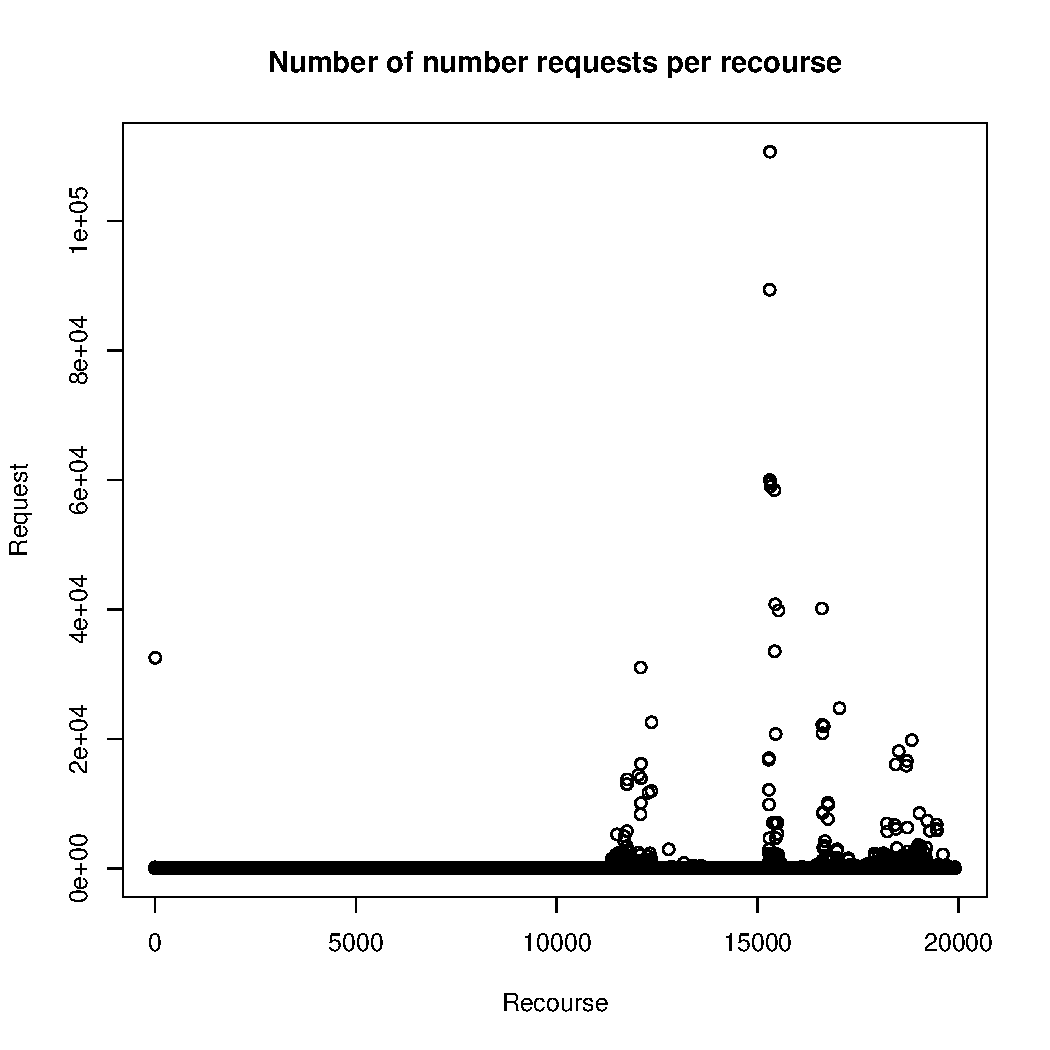
\includegraphics[scale=0.95]{Weblogs/Jul/NumberOfNumberRequestsPerRecourse.pdf}}
\caption{Number of requests per resource, July}
\end{figure}
The most popular request is the small logo of NASA with address /images/NASA-logosmall.gif\footnote{output of weblogsMode(weblogs\$Request)}. NASA server provided an access to the resources 9684\footnote{output of mostFriqAmount(weblogs\$Request)} times in July and 110679 in August.\\ The most popular resource is significantly higher than other ones, probably the logo is placed at the most part of the NASA webpages.
\begin{figure}[H]
\centerline{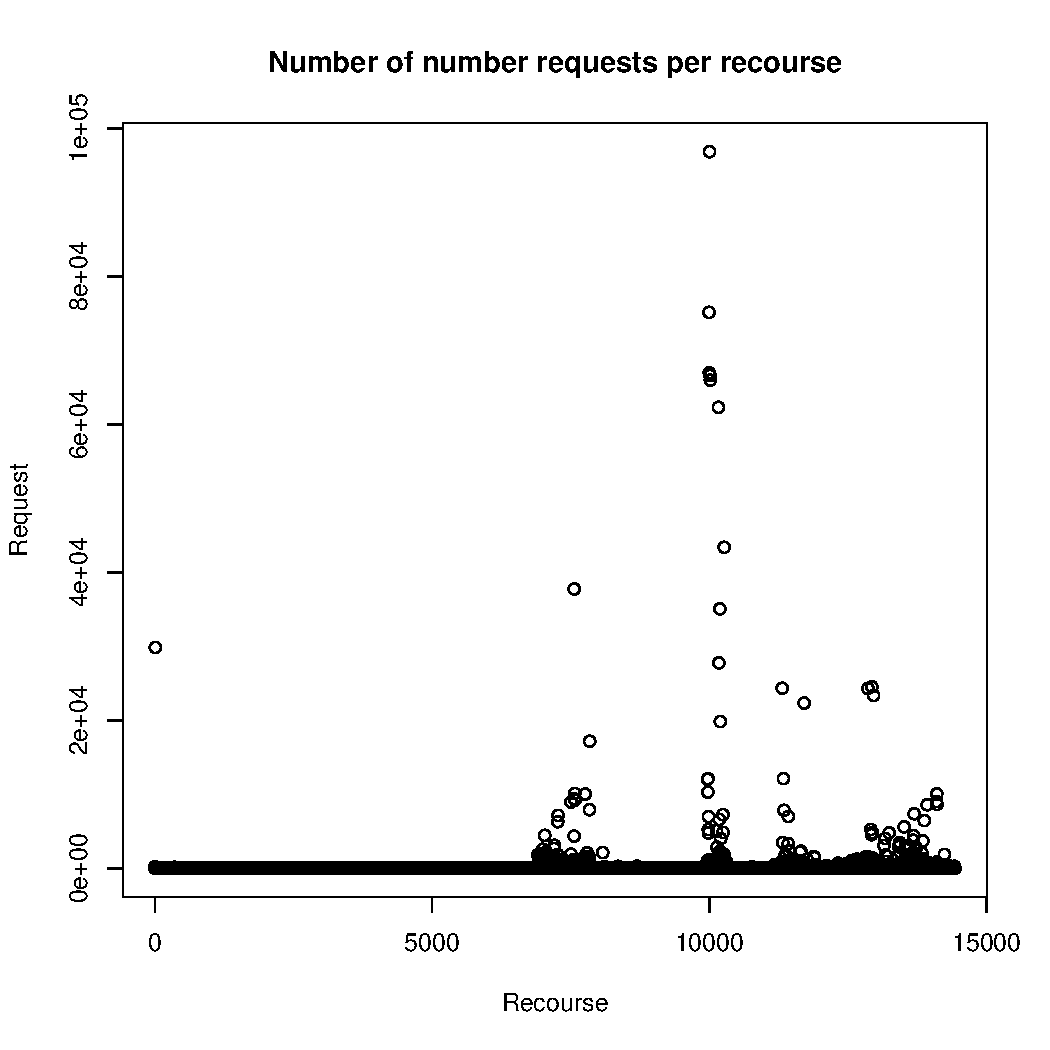
\includegraphics{Weblogs/Aug/NumberOfNumberRequestsPerRecourse.pdf}}
\caption{Number of requests per resource, August}
\end{figure}



\subsubsection{The second most popular resource}
I compared the sum of requests to the most popular resources for different days and number of requests to NASA-logosmall and found that they are not same. It means that there are several days when other resource is more popular. It is other logo with address /images/KSC-logosmall.gif, the most popular resources for different days are represented in a table 3\footnote{output of mostPupolarRequestOfDay(weblogs)}.
\begin{table}[H]
\caption{The most popular resource of day}
\centerline{
\begin{tabular}{lll}
\hline
day &  July & August \\
\hline
1&/images/NASA-logosmall.gif& - \\
2&/images/NASA-logosmall.gif&- \\
3&/images/NASA-logosmall.gif&-\\
4&/images/NASA-logosmall.gif&/images/NASA-logosmall.gif\\
5&/images/KSC-logosmall.gif&/images/NASA-logosmall.gif\\
6&/images/NASA-logosmall.gif&/images/NASA-logosmall.gif\\
7&/images/NASA-logosmall.gif&/images/NASA-logosmall.gif\\
8&/images/NASA-logosmall.gif&/images/NASA-logosmall.gif\\
9&/images/NASA-logosmall.gif&/images/NASA-logosmall.gif\\
10&/images/NASA-logosmall.gif&/images/NASA-logosmall.gif\\
11&/images/KSC-logosmall.gif&/images/NASA-logosmall.gif\\
12&/images/KSC-logosmall.gif&/images/NASA-logosmall.gif\\
13&/images/NASA-logosmall.gif&/images/NASA-logosmall.gif\\
14&/images/NASA-logosmall.gif&/images/NASA-logosmall.gif\\
15&/images/NASA-logosmall.gif&/images/NASA-logosmall.gif\\
16&/images/NASA-logosmall.gif&/images/NASA-logosmall.gif\\
17&/images/NASA-logosmall.gif&/images/NASA-logosmall.gif\\
18&/images/KSC-logosmall.gif&/images/KSC-logosmall.gif\\
19&/images/KSC-logosmall.gif&/images/KSC-logosmall.gif\\
20&/images/NASA-logosmall.gif&/images/NASA-logosmall.gif\\
21&/images/NASA-logosmall.gif&/images/NASA-logosmall.gif\\
22&/images/NASA-logosmall.gif&/images/NASA-logosmall.gif\\
23&/images/NASA-logosmall.gif&/images/NASA-logosmall.gif\\
24&/images/NASA-logosmall.gif&/images/KSC-logosmall.gif\\
25&/images/KSC-logosmall.gif&/images/KSC-logosmall.gif\\
26&/images/KSC-logosmall.gif&/images/KSC-logosmall.gif\\
27&/images/NASA-logosmall.gif&/images/NASA-logosmall.gif\\
28&/images/NASA-logosmall.gif&/images/NASA-logosmall.gif\\
29&/images/NASA-logosmall.gif&/images/NASA-logosmall.gif\\
30&/images/NASA-logosmall.gif&/images/NASA-logosmall.gif\\
31&/images/NASA-logosmall.gif&/images/NASA-logosmall.gif\\
\end{tabular}}
\end{table}


It seems to be that there is a correlation between holidays and days when KSC-logosmall.gif is more popular than NASA-logosmall, in most cases it follows pattern: five days NASA-logosmall.gif and two days KSC-logosmall.gif. \\\\
But it is false correlation, because both of them are actually related to the number of requests per day. The figures 3 and 4\footnote{plots of outputs of the function requestsPerDay(weblogs)} shows us that KSC-logosmall is more popular than NASA-logosmall at day with relatively low amount of requests to the server and at the same times in the number of requests usually is low at holidays.\\\\
It is possible to clearly identify days of week with graphs below, by couples of days with relatively low amount of requests.


\begin{figure}[H]
\centerline{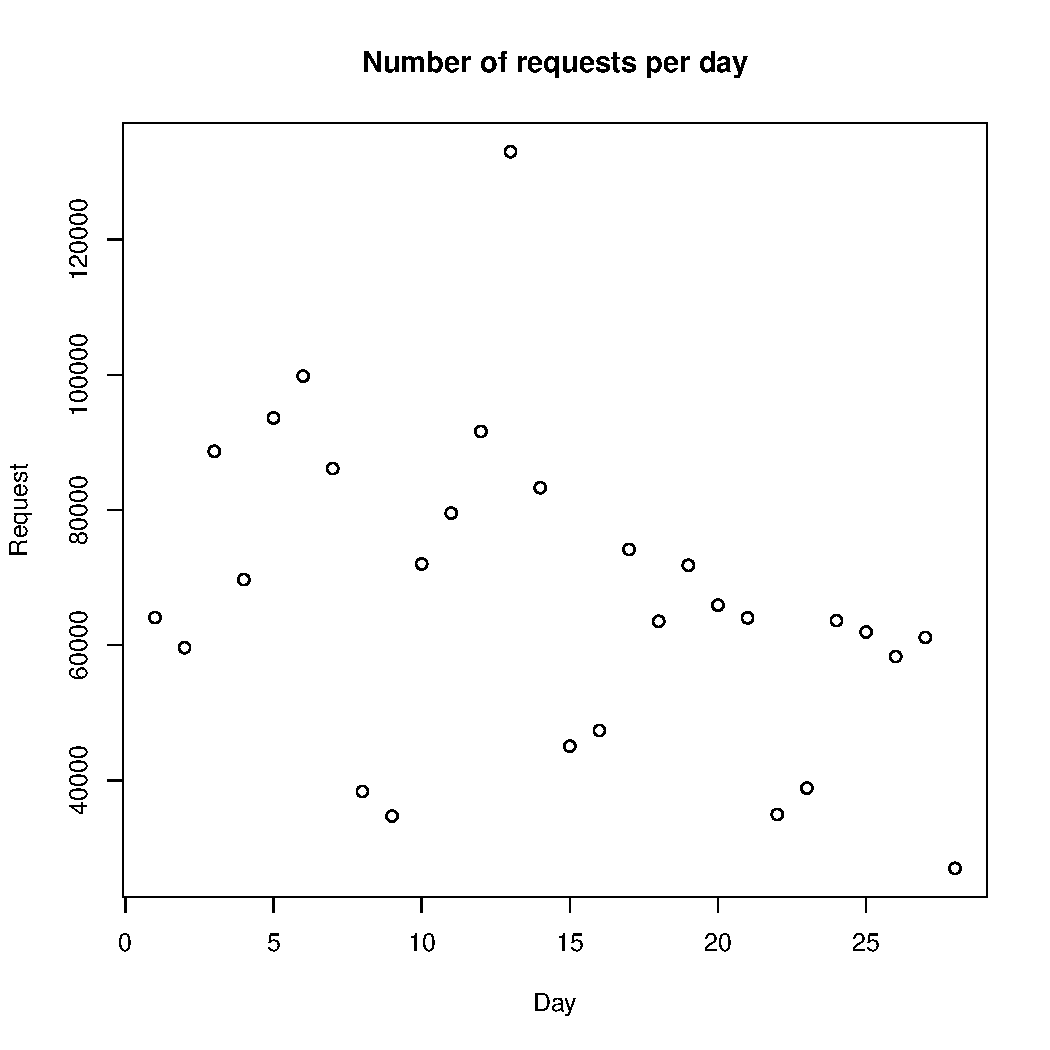
\includegraphics{Weblogs/Jul/NumberOfRequestsPerDay.pdf}}
\caption{Number of requests per day, July}
\end{figure}
The smallest number of requests per day is 31180 in July and 26970 in August, the biggest values are 89330, 133000 and average numbers of requests for the months are 51860 and 66860, total average is 59098.52.
\begin{figure}[H]
\centerline{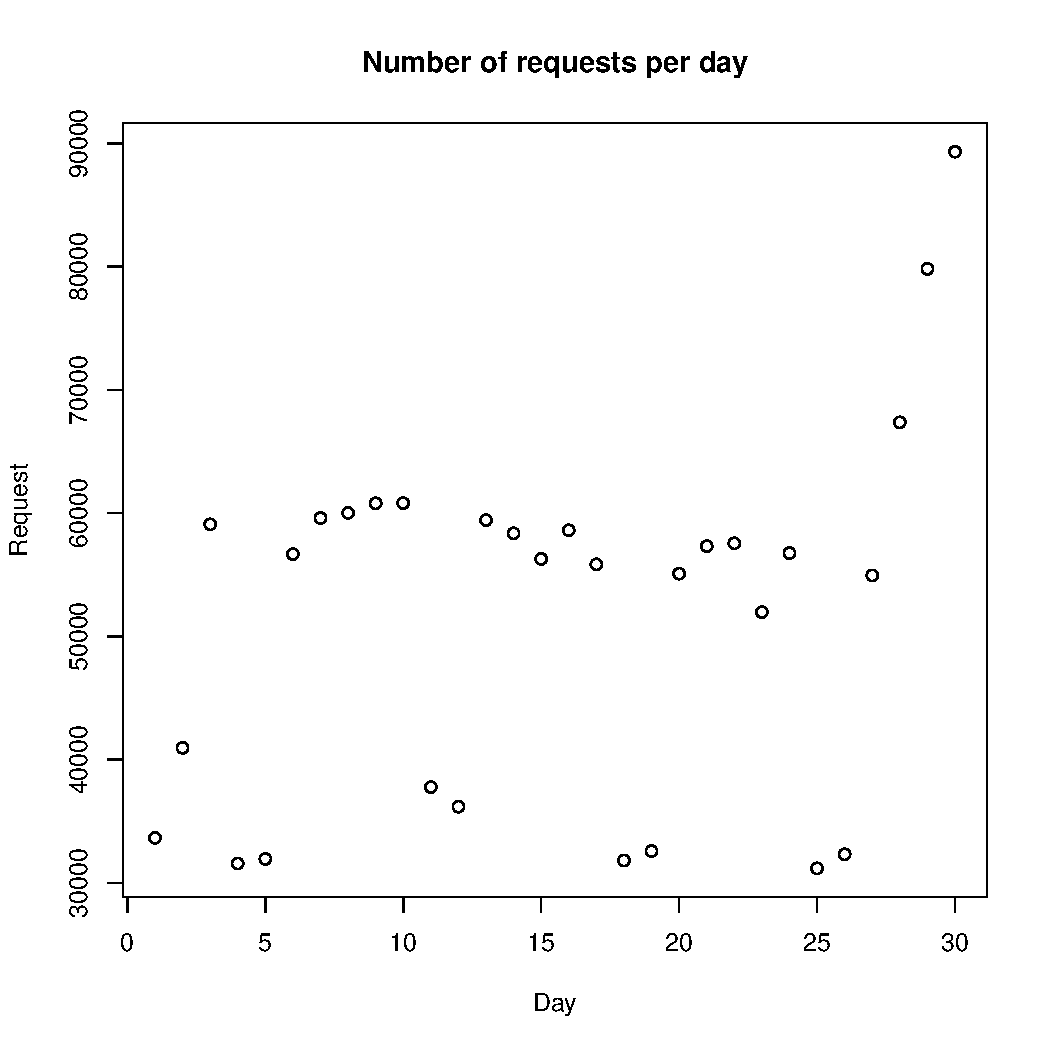
\includegraphics{Weblogs/Aug/NumberOfRequestsPerDay.pdf}}
\caption{Number of requests per day, August}
\end{figure}




\subsubsection{Most popular requests per day}
Most popular resources are requested from 1472 to 8343 times a day in July and from 1458 to 12050 in August. An average amount number of requests to the most popular resource of the day is  3254 for July and 3977 for August, total mean is 3603. The information about the number of requests to the most popular resources of day is represented in graphs number 5 and 6.\footnote{the data is output of mostPupolarRequestOfDayAmount(weblogs)}
\begin{figure}[H]
\centerline{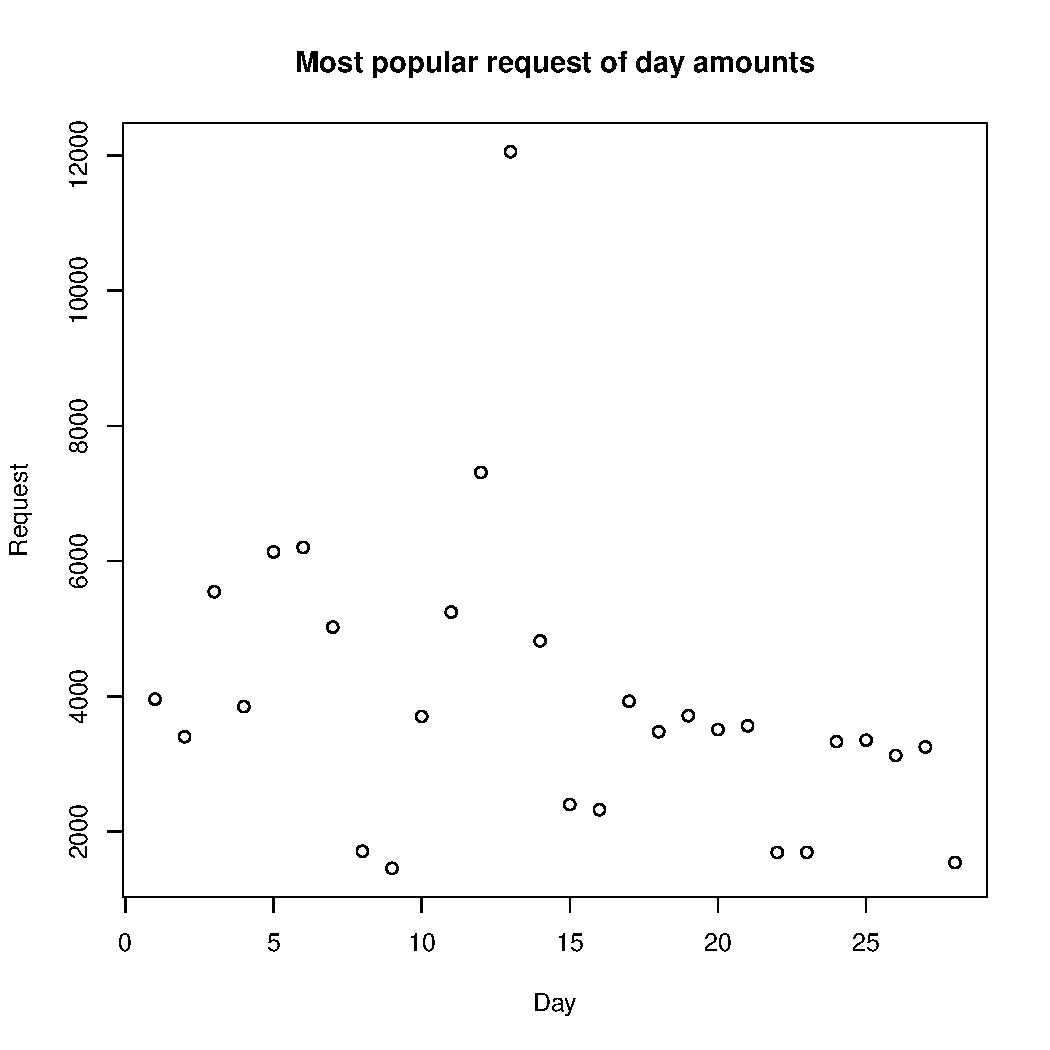
\includegraphics{Weblogs/Jul/MostPopularRequestOfDayAmounts.pdf}}
\caption{Number of the requests to the most popular resource per days, July}
\end{figure}
\begin{figure}[H]
\centerline{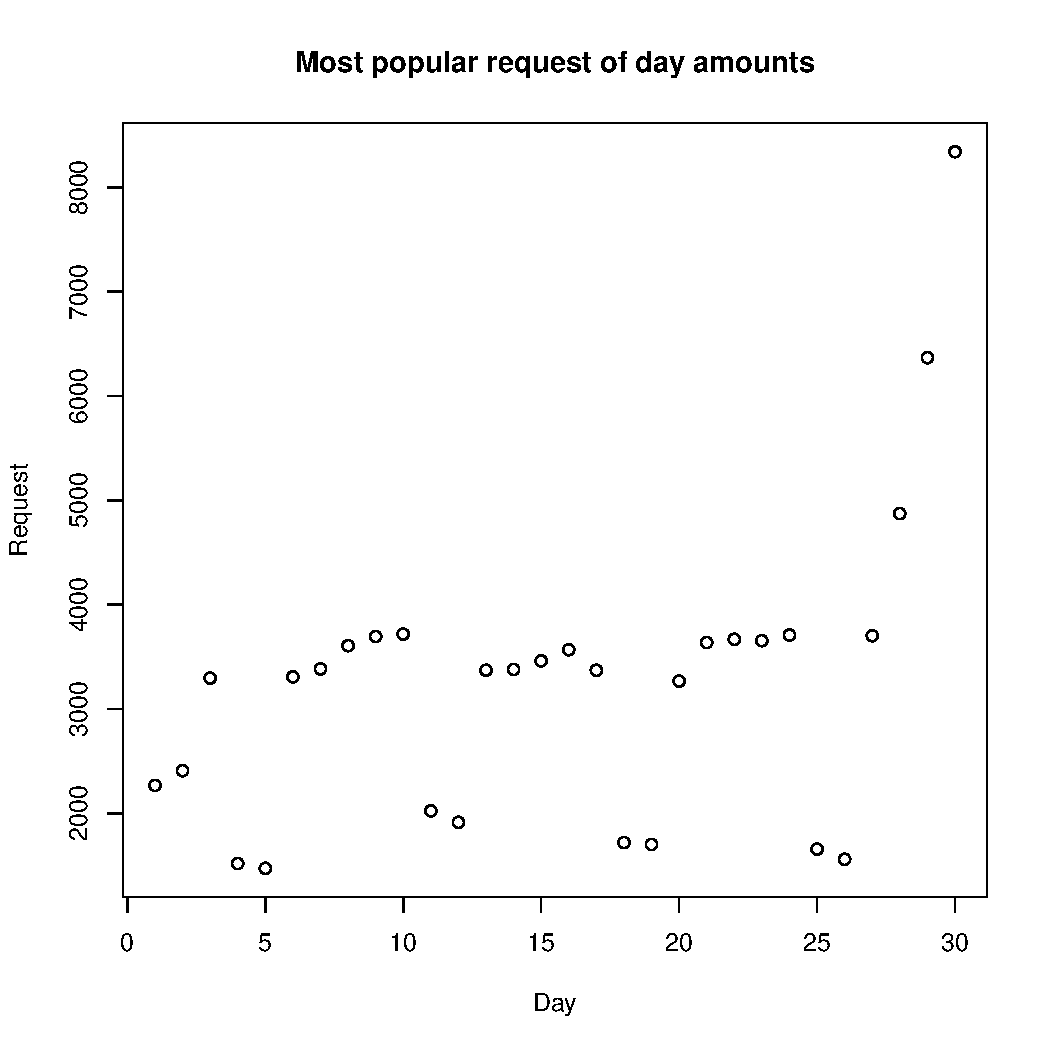
\includegraphics{Weblogs/Aug/MostPopularRequestOfDayAmounts.pdf}}
\caption{Number of the requests to the most popular resource per days, August}
\end{figure}



\subsection{Users or Hosts}
The website had 74810 users in July and 81625 in August. Figures 7,8\footnote{plots of outputs of the function hostsPerDay(weblogs)} demonstrates that number of user during month per days, obviously, follows the same structure as the number of requests per day, because more users produce more requests.
\begin{figure}[H]
\centerline{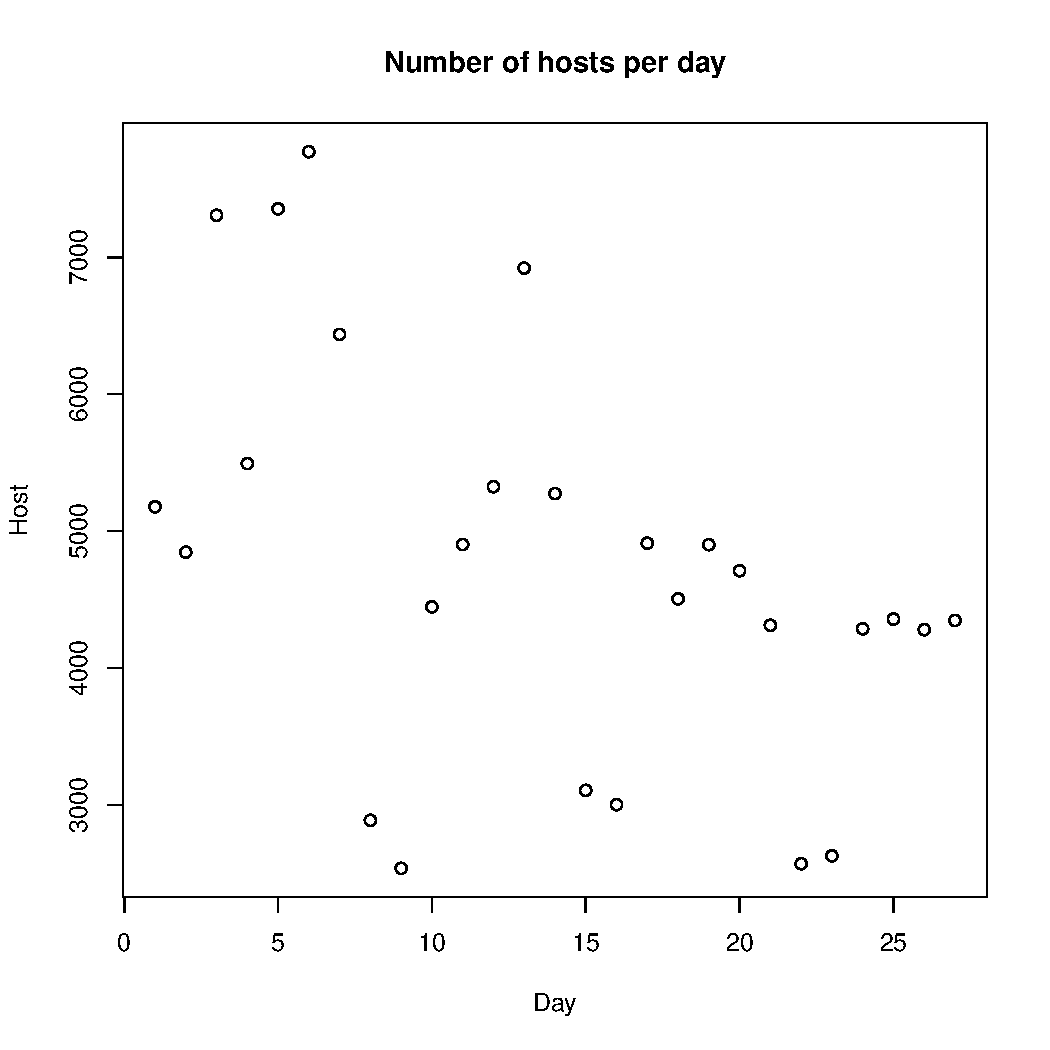
\includegraphics{Weblogs/Jul/NumberOfHostsPerDay.pdf}}
\caption{Number of users per day, July}
\end{figure}
The biggest number of users per day were 5253 in July and 7772 in August, the smallest were 2492 and 2536, average amount of users per day were 3781 and 4763, total average was 4254.
\begin{figure}[H]
\centerline{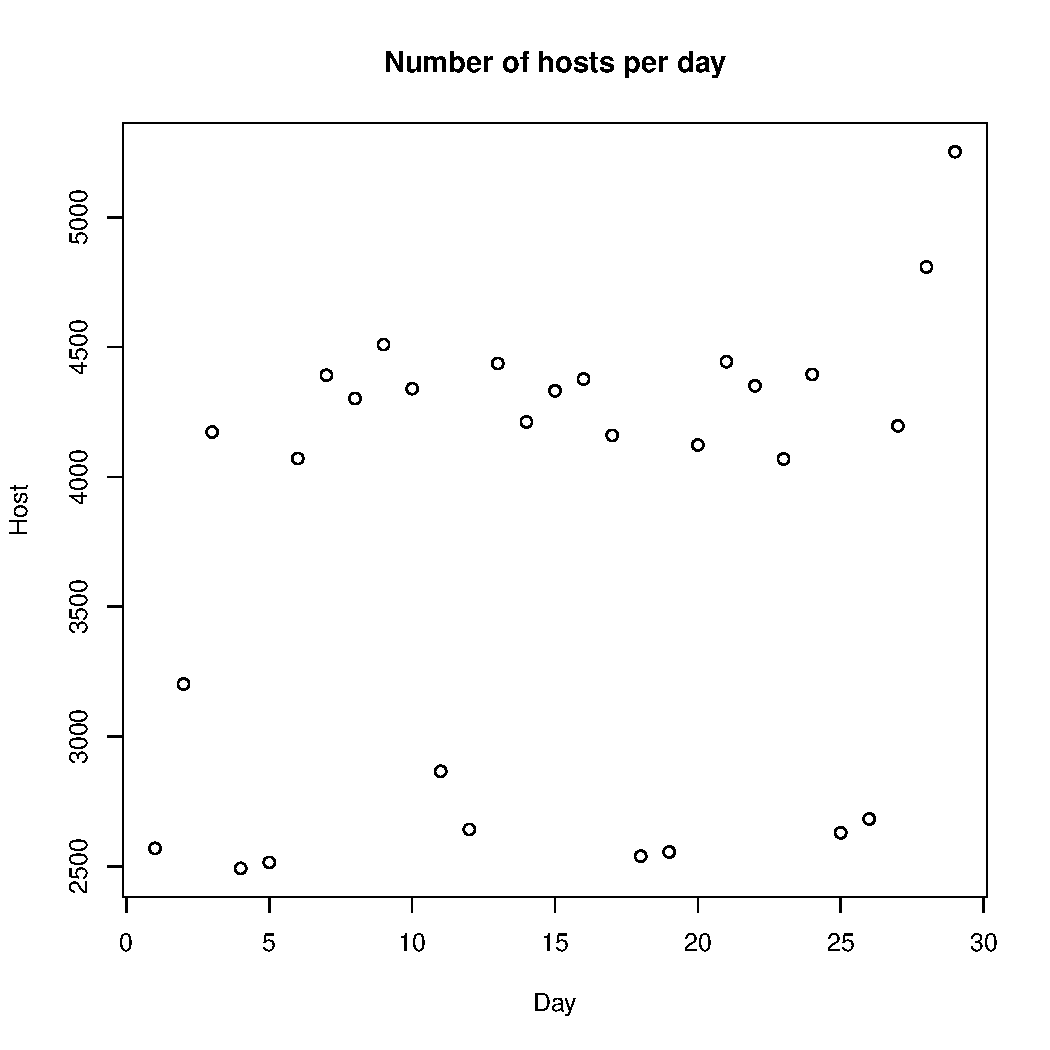
\includegraphics{Weblogs/Aug/NumberOfHostsPerDay.pdf}}
\caption{Number of users per day, August}
\end{figure}



\subsubsection{Requests per user}
The most active users are  piweba3y.prodigy.com with 17382 requests in July and edams.ksc.nasa.gov with 6515, in August, but there are also plenty other active hosts during months on the table 4.
\begin{table}[H]
\caption{The most active Host of day}
\centerline{
\begin{tabular}{lll}
\hline
day &  July & August \\
\hline
1&edams.ksc.nasa.gov& - \\
2&gn2.getnet.com&- \\
3&163.205.156.16&-\\
4&piweba5y.prodigy.com&piweba3y.prodigy.com\\
5&bnl871c.ags.bnl.gov&piweba3y.prodigy.com\\
6&quadra\_echo.rollins.edu&piweba3y.prodigy.com\\
7&lsda05.jsc.nasa.gov&piweba3y.prodigy.com\\
8&163.206.89.4&news.ti.com\\
9&bambi.te.rl.ac.uk&piweba3y.prodigy.com\\
10&news.ti.com&piweba3y.prodigy.com\\
11&206.27.25.1&piweba3y.prodigy.com\\
12&198.83.19.44&alyssa.prodigy.com\\
13&128.32.196.94&e659229.boeing.com\\
14&pc24.ac.tandem.com&bill.ksc.nasa.gov\\
15&piweba3y.prodigy.com&indy.gradient.com\\
16&139.169.174.102&piweba3y.prodigy.com\\
17&141.102.82.127&piweba4y.prodigy.com\\
18&rmcg.cts.com&piweba4y.prodigy.com\\
19&piweba4y.prodigy.com&piweba3y.prodigy.com\\
20&e659229.boeing.com&siltb10.orl.mmc.com\\
21&edams.ksc.nasa.gov&siltb10.orl.mmc.com\\
22&128.217.62.2&siltb10.orl.mmc.com\\
23&edams.ksc.nasa.gov&siltb10.orl.mmc.com\\
24&mac998.kip.apple.com&siltb10.orl.mmc.com\\
25&silver.tiac.net&currypc.fpl.msstate.edu\\
26&piweba5y.prodigy.com&currypc.fpl.msstate.edu\\
27&j70mgs.kav.magwien.gv.at&198.133.29.18\\
28&163.206.89.4&jbiagioni.npt.nuwc.navy.mil\\
29&beta.xerox.com&piweba3y.prodigy.com\\
30&beta.xerox.com&edams.ksc.nasa.gov\\
31&edams.ksc.nasa.gov&pcmas.it.bton.ac.uk\\
\end{tabular}}
\end{table}

\begin{figure}[H]
\centerline{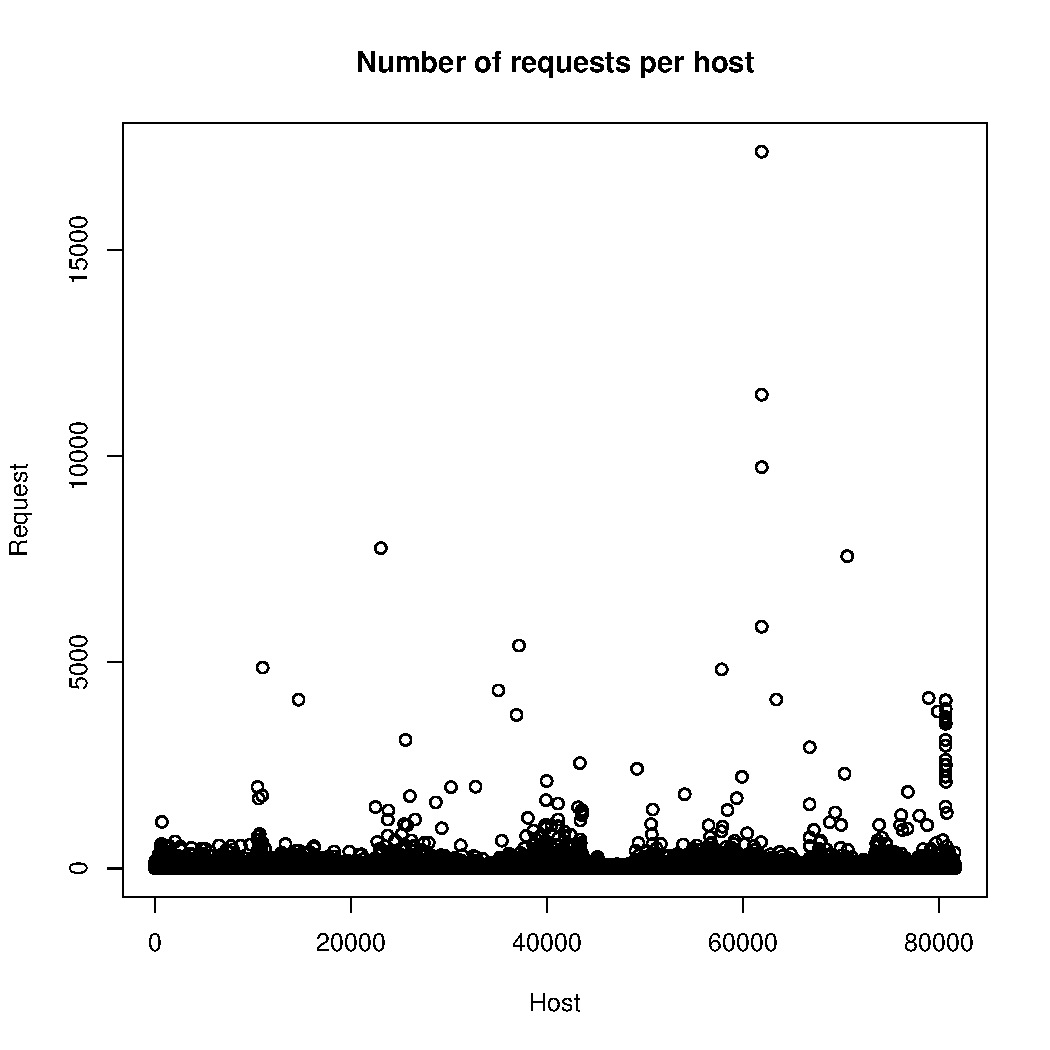
\includegraphics{Weblogs/Jul/NumberOfRequestsPerhost.pdf}}
\caption{Number of requests users per user, July}
\end{figure}
\begin{figure}[H]
\centerline{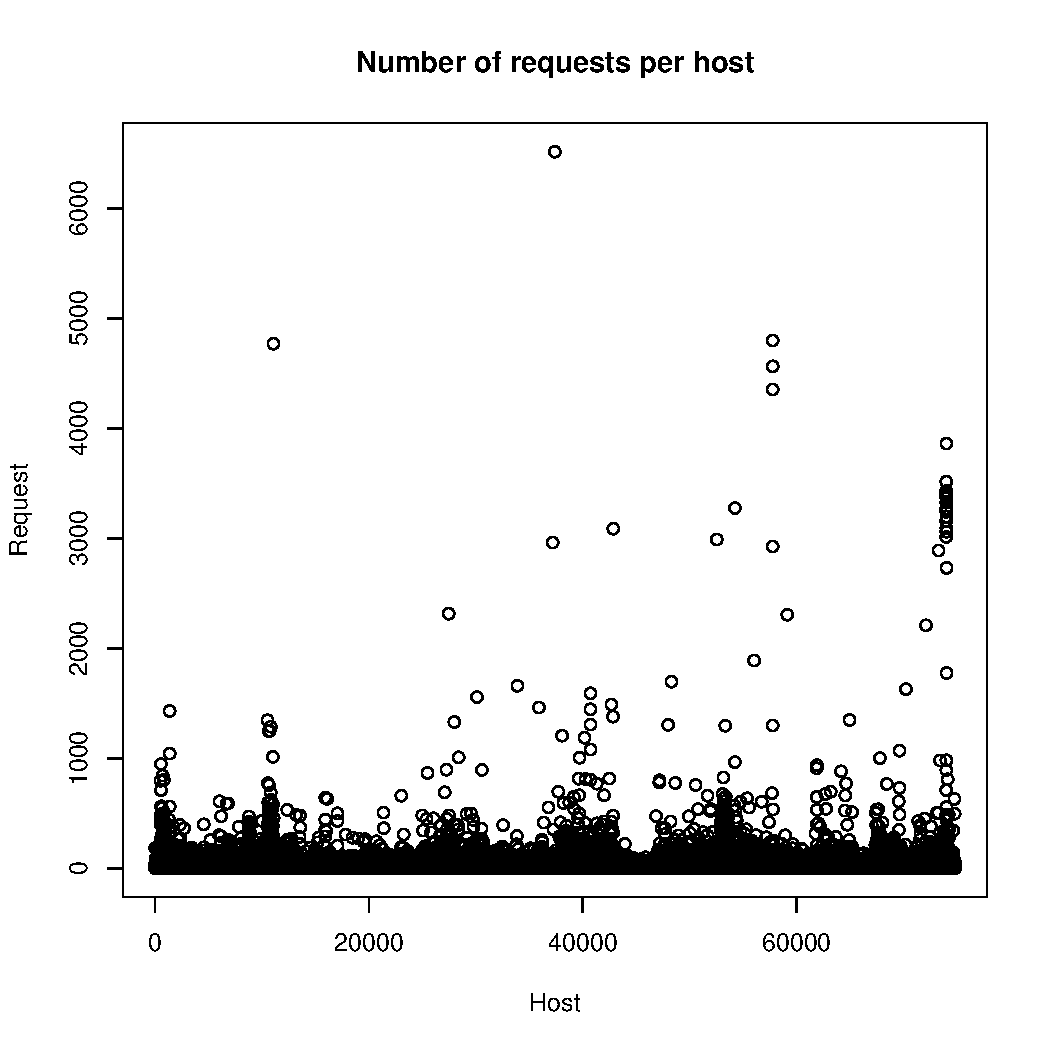
\includegraphics{Weblogs/Aug/NumberOfRequestsPerhost.pdf}}
\caption{Number of requests users per user, August}
\end{figure}
\subsubsection{Most active hosts}
Most active hosts made from 195 to 1113 requests per day in July and from 282 to 1391 in August. An average amount of requests from the most active user of the day is  438 for July and 821 for August, total mean is 622.7. The information about number of requests from the most active hosts of day is represented in a graph number 11 and 12.\footnote{the data is output of mostActiveHostOfDayAmount(weblogs)}
\begin{figure}[H]
\centerline{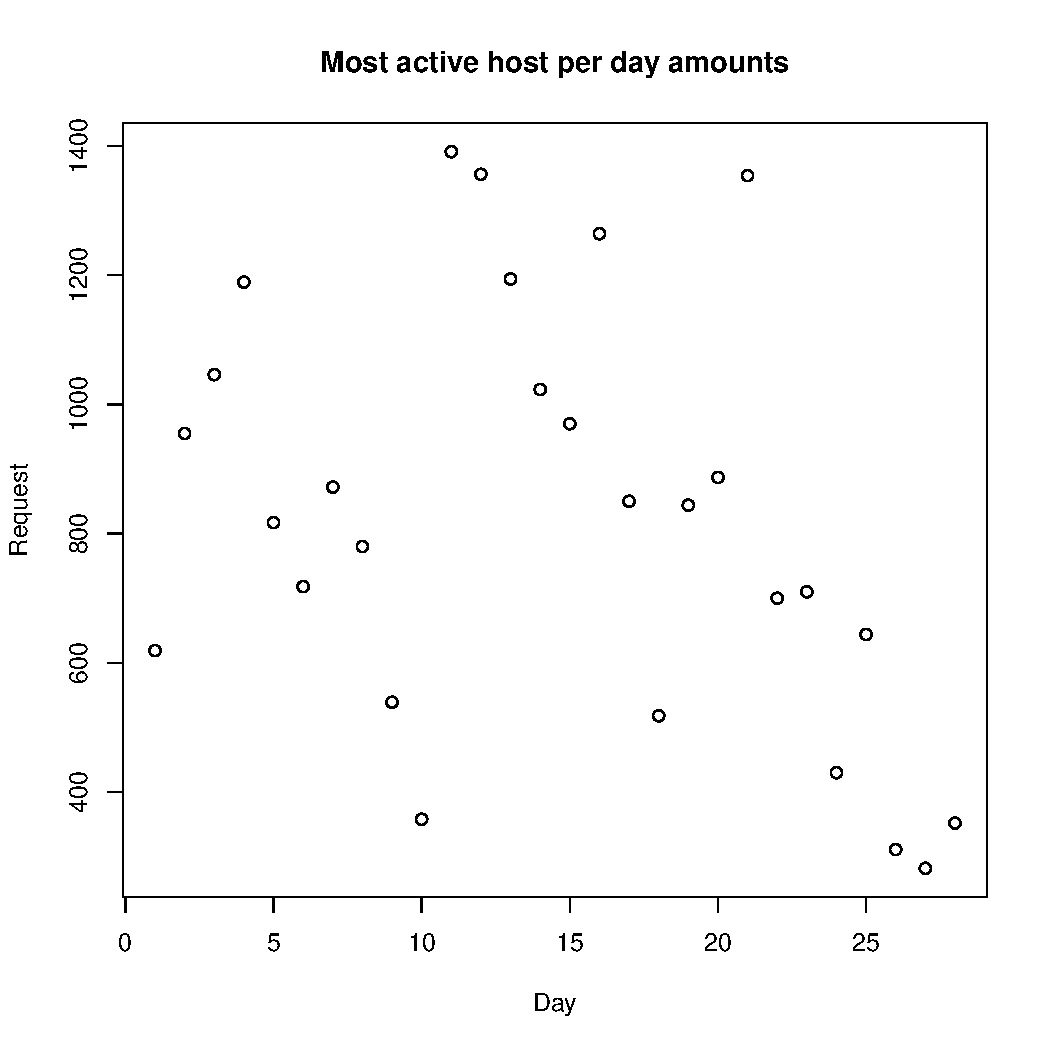
\includegraphics{Weblogs/Jul/MostActiveHostPerDayAmounts.pdf}}
\caption{Number of the requests from the most active host of day, July}
\end{figure}
\begin{figure}[H]
\centerline{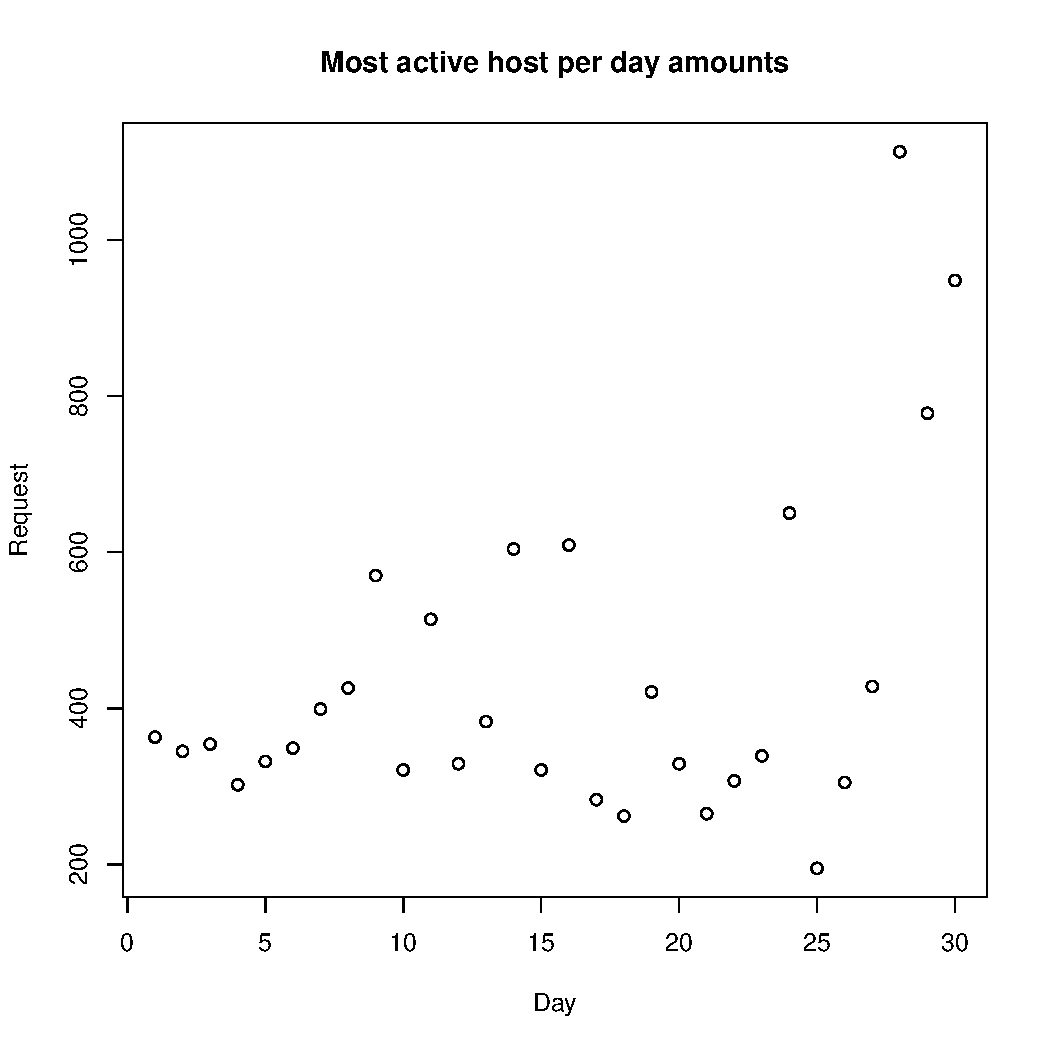
\includegraphics{Weblogs/Aug/MostActiveHostPerDayAmounts.pdf}}
\caption{Number of the requests from the most active host of day, August}
\end{figure}
\subsection{Data}
Server had sent 3198.187MB\footnote{26828341054 bytes, output of dataAmount(weblogs)} of data in July and 4612.783MB\footnote{38694831788 bytes} in August, the biggest response was 417.7183KB\footnote{3421948 bytes, output of max(as.numeric(as.character(weblogs\$Bytes))} and  833KB\footnote{6823936 bytes}, average 2.1KB\footnote{17240 bytes, output of summary(as.numeric(as.character(weblogs\$Bytes))} and 2.5KB\footnote{20670 bytes}.
\begin{figure}[H]
\centerline{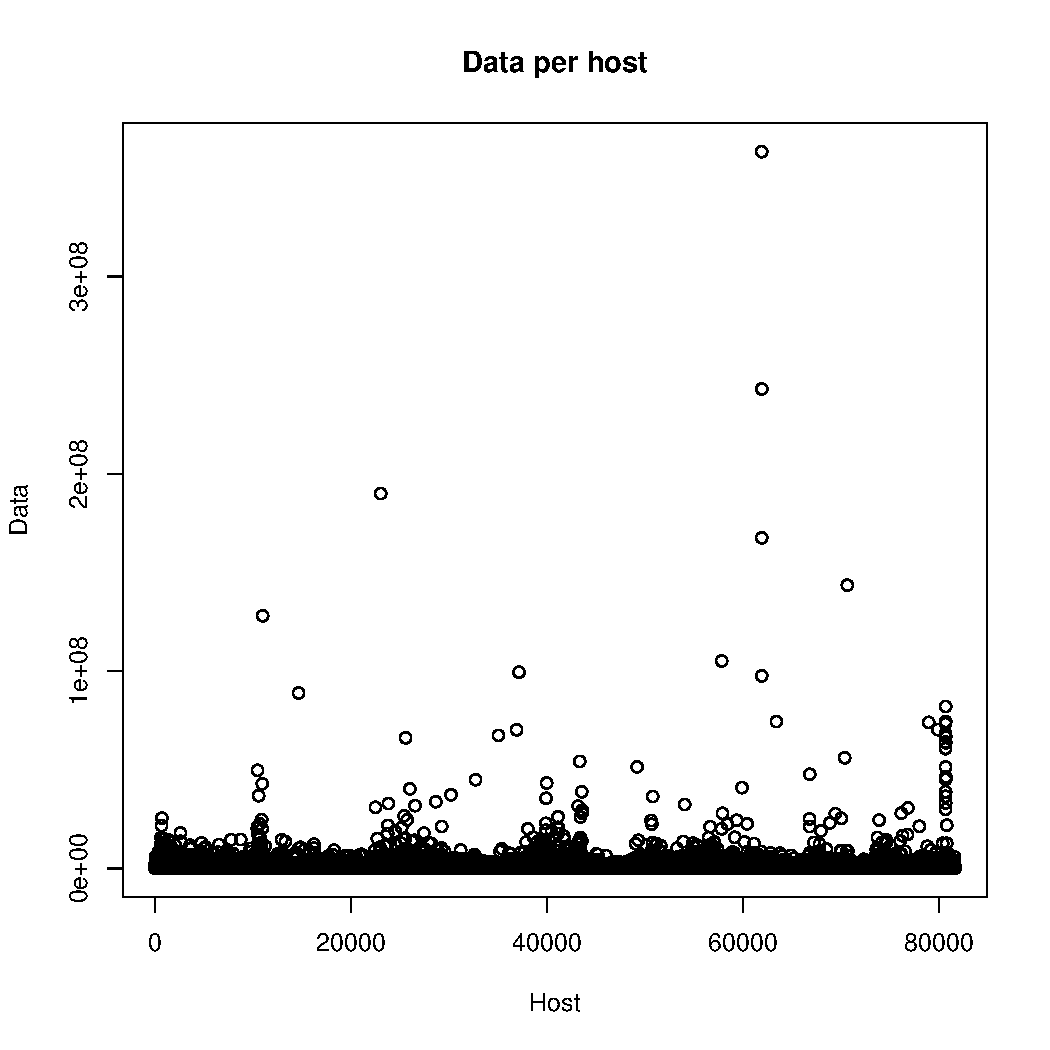
\includegraphics{Weblogs/Jul/DataPerHost.pdf}}
\caption{Number of bytes per host, July}
\end{figure}
Users received 41.6KB\footnote{341100 bytes, output of summary(dataPerHost(weblogs))} and 55.4KB\footnote{453700 bytes}in average. The most active hosts received 13MB\footnote{108900000 bytes, output of summary(dataPerHost(a))} and 43MB\footnote{363300000 bytes} in July and August, correspondingly.
Obviously, amount of data per host has the same pattern as number of requests per host.
\begin{figure}[H]
\centerline{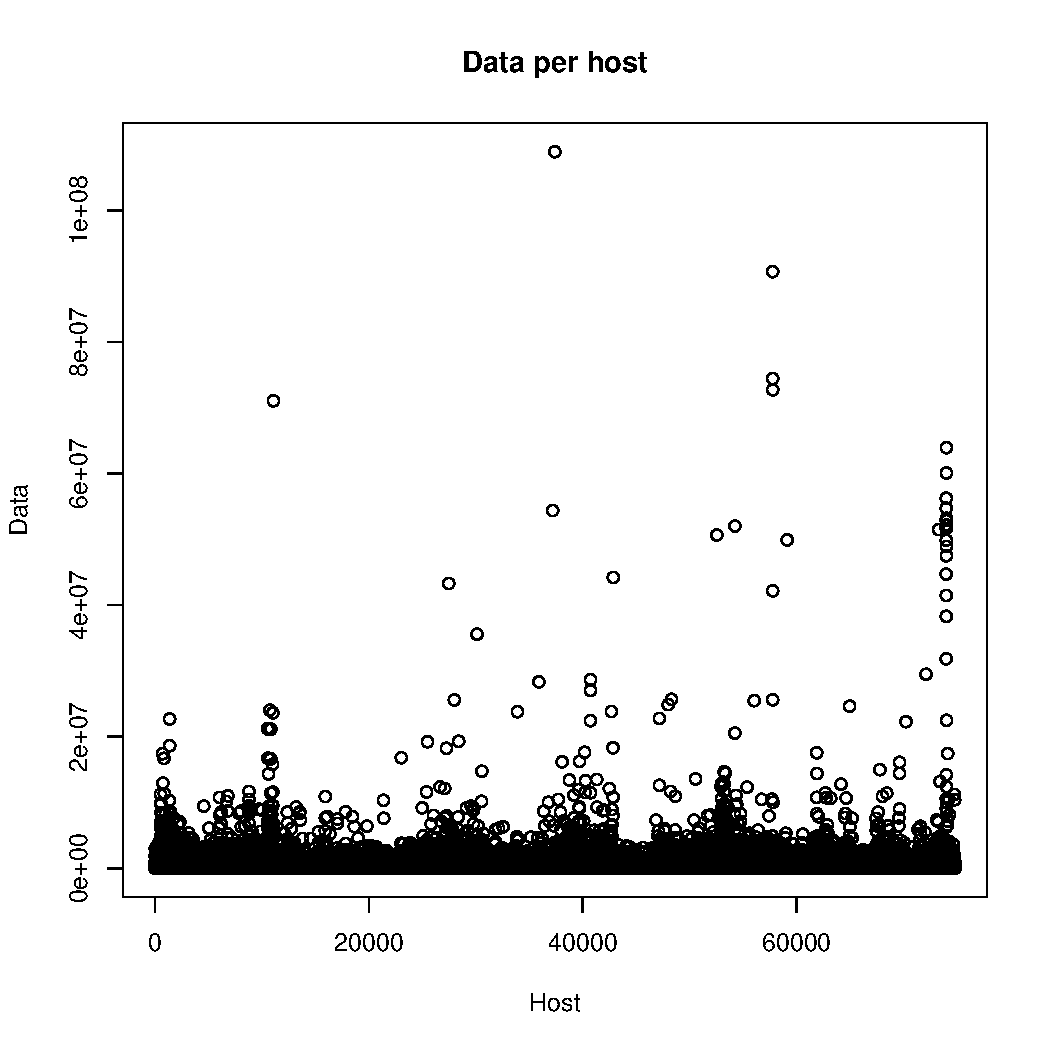
\includegraphics{Weblogs/Aug/DataPerHost.pdf}}
\caption{Number of bytes per host, August}
\end{figure}
The amount of transferred data per day follows general pattern as number of requests per day and number of hosts per day.(Figures 13, 14)
\begin{figure}[H]
\centerline{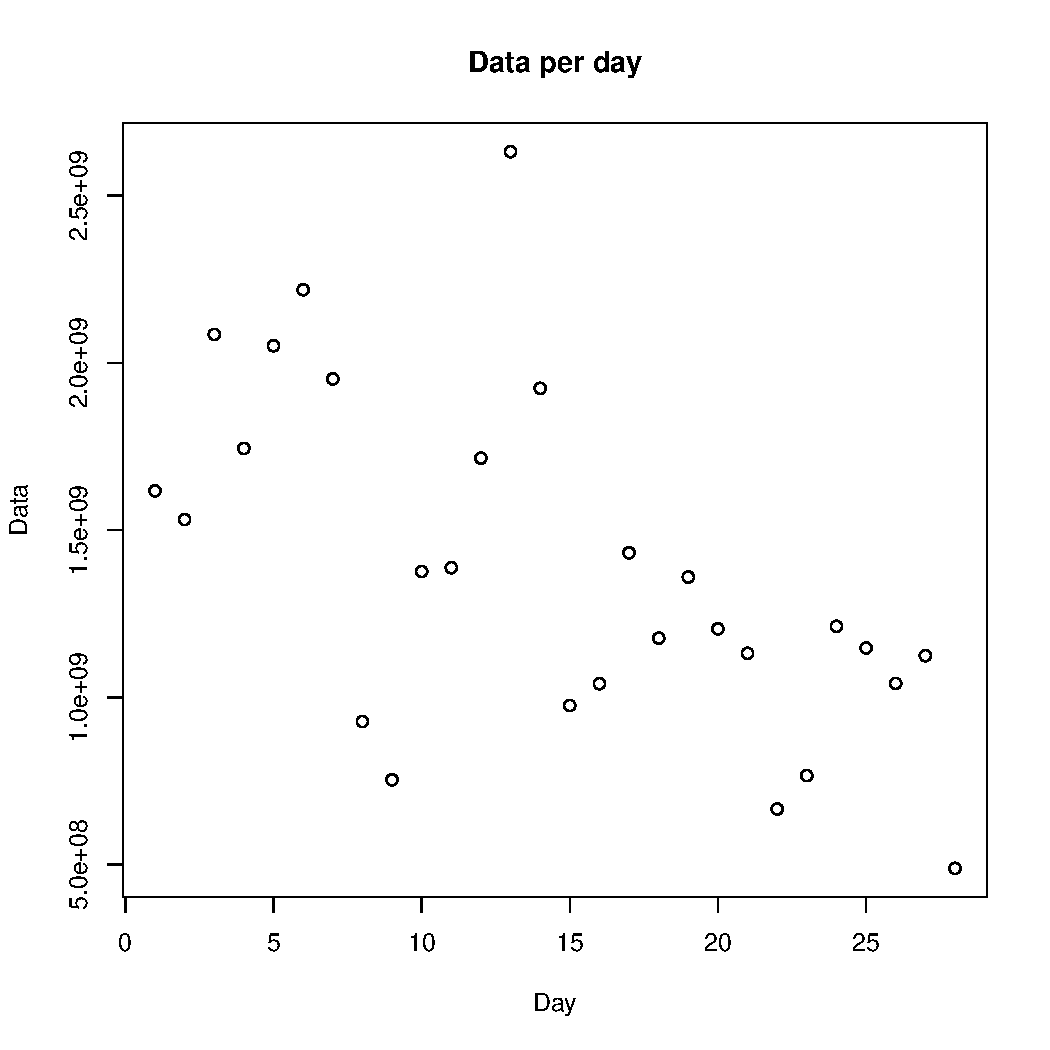
\includegraphics{Weblogs/Jul/DataPerDay.pdf}}
\caption{Amount of data per days, July}
\end{figure}
\begin{figure}[H]
\centerline{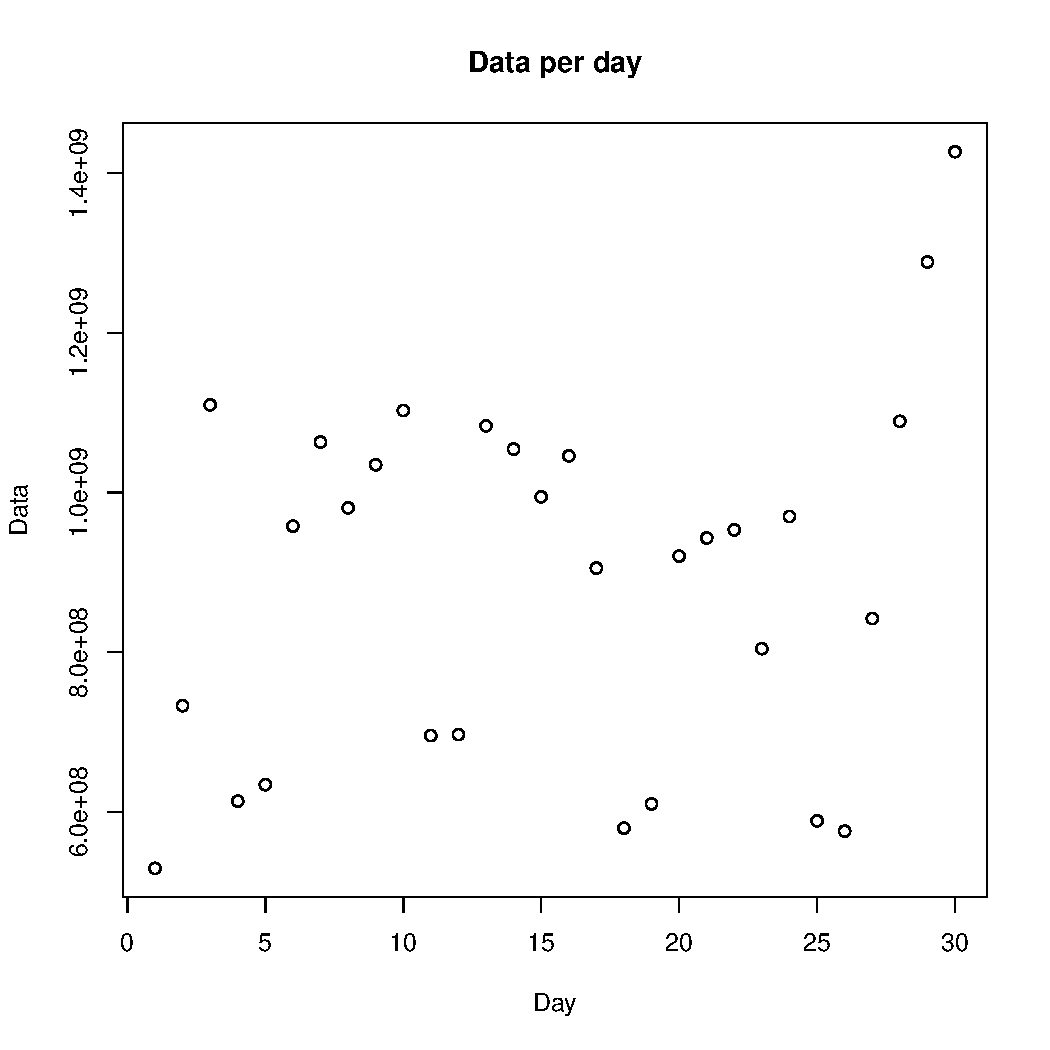
\includegraphics{Weblogs/Aug/DataPerDay.pdf}}
\caption{Amount of data per days, August}
\end{figure}

\section{Linear regression}
Linear regression is a statistical technical very popular for modelling of relationship between two or more variables. Linear regression with only one explanatory variable is called Simple Linear Regression.\\\\
An output of linear regression is formed by linear predictor function and this kind of models is often called linear model. In case of simple linear regression linear predictor function is actually just a linear function.
\subsection{Simple linear regression}
Amount of data per day\footnote{output of dataAmountPerDay(weblogs)} is depended from amount of requests\footnote{output of requestsPerDay(weblogs)}, the idea is proofed by the fact that the graphs on fig. 3 and fig. 15 have very similar pattern. Probably it is possible to use simple linear regression to predict an amount data transferred by number o requests at the day. 

\begin{figure}[H]
\centerline{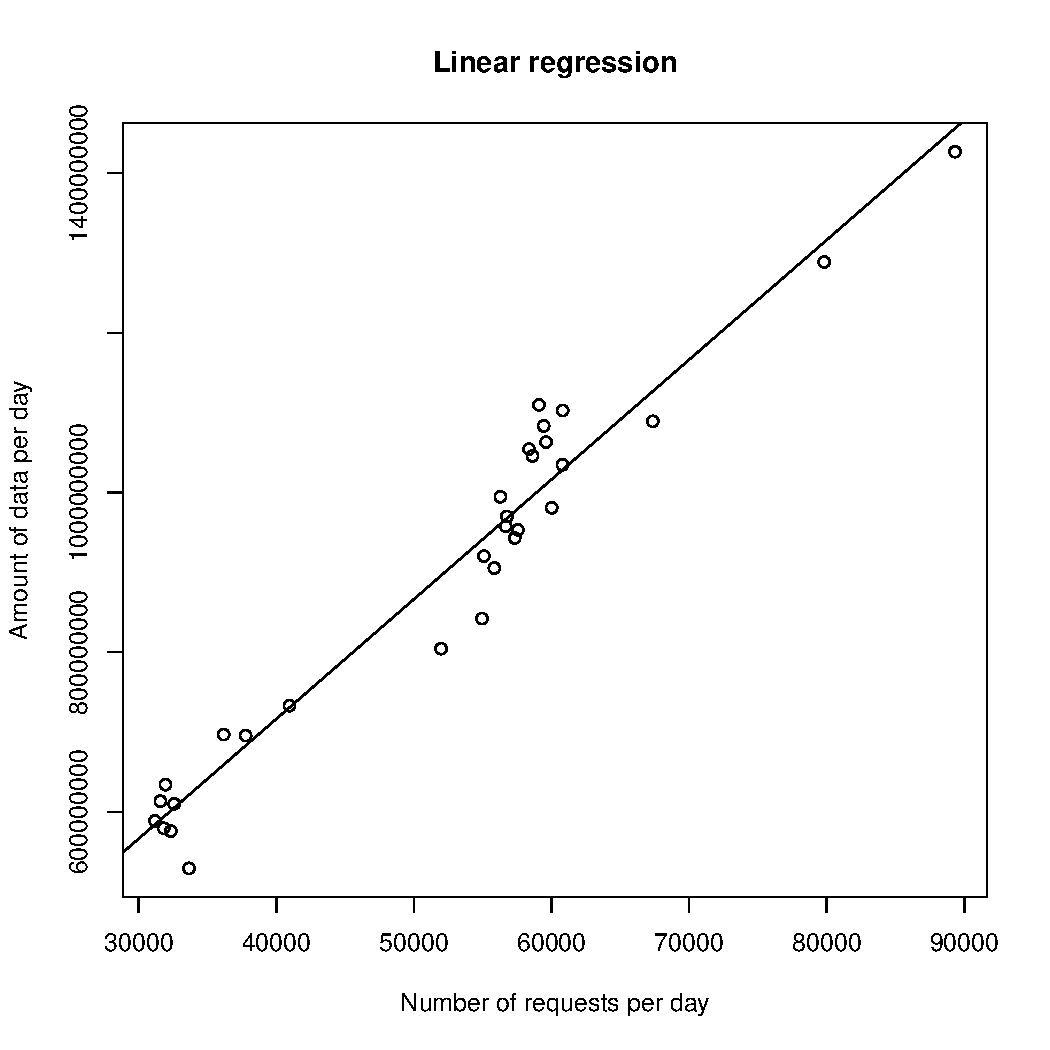
\includegraphics{Weblogs/LiniarReg.pdf}}
\caption{Dependence of transfered data from amount of requests}
\end{figure}
\subsubsection{Simple model for July}
The values have correlation coefficient 0.975 and it means that the result would be very accurate.
Graph on fig. 17 shows the relationships between the sets and all of the dots are situated quite close to the trend line.\\\\

As I already noticed simple linear regression use linear function as predictor function so, lm function gives us $k=14995.69$ and $b=116605001.33$ for training data based on July.\\\\
Testing of the model with data from the same month gives me average error 4.5\%, smallest error is 0.23\% and the biggest one is 17\%, but it is not so accurate for data from other month the model gives us mean 16\%, minimal error is 3.8\% and maximal one is 34\%.\\
Mean error for both datasets is 10.5\%.
\begin{table}[H]
\caption{Errors for different test for model based on July}
\centerline{
\begin{tabular}{lccc}
\hline
&  Smallest & Average & Biggest \\
\hline
July &  0.23\% & 4.5\% & 17\%\\
August & 3.8\% &16\% & 34\% \\
Whole datum &   0.23\% & 10.5\% & 34\%
\end{tabular}}
\end{table}
\subsubsection{Simple model for August}
Correlation between the values is lower, only 0.943, it means linear regression model will be less successful.\\\\
Linear function for model based on data from August has $b=-15731021.1$ and $k=20905.39 $. So, the model has very big average error even for a test with a data from this month, it is 10.7\%, the smallest error is 3.8\% and the biggest one is 19\%.\\\\
The models gives the smallest error 2.8\%, average 18.5\% and 34.5\% for July.\\\\
Average error for whole datum is 14\%.
So, July's model is more successful.
\begin{table}[H]
\caption{Errors for different tests for model based on August}
\centerline{
\begin{tabular}{lccc}
\hline
&  Smallest & Average & Biggest \\
\hline
July &  2.8\% & 18.5\% & 34.5\%\\
August & 3.8\% &10.7\% & 19\% \\
Whole datum &   2.8\% & 14\%. & 34.5\%
\end{tabular}}
\end{table}
\subsubsection{Simple model for whole datum}
Together both months have even lower correlation than August, it is 0.935.\\\\
Model for this dataset contains $k=20915$ and $b=-106376328.1$.\\\\
So, an average error for the model for the both months is 10.6\%. \\\\
The smallest error for July is 1\%, an average is 10.9\% and the biggest is 23.8\%.\\\\
For August the model works even better than native one and gives the smallest error 0.8\%, an average is 10.2\% and only biggest one is worse, 25.5\%.
\begin{table}[H]
\caption{Errors for different test for model based on July}
\centerline{
\begin{tabular}{lccc}
\hline
&  Smallest & Average & Biggest \\
\hline
July &  1\% & 10.9\% & 23.8\%\\
August & 3.8\% &16\% & 34\% \\
Whole datum &   0.8\% & 10.2\%.&25.5\%
\end{tabular}}
\end{table}
\subsection{Multiple Linear regression}
Linear regression with several explanatory variables is called Multiple-Linear Regression, it can be more stable than simple one. In linear predict function for multiple linear regression every explanatory variable has their own coefficient.\\\\
I am going to use amount of users per day as second explanatory variable.\\\\
Correlation between number of hosts per day\footnote{output of hostsPerDay(weblogs)} and amount of transmitted data is 0.96.
\subsubsection{Multiple Linear regression for July}

The Multiple Linear regression models I tested only on full datum. So average error is 10\%, smallest is smaller than 0.001 and biggest is 35\%. 
I decided that I will not make model for August because the simple linear regression for this part of data was the worst.
$$k_{requests}=17893.73$$$$ k_{hosts}=-46837.01$$$$b=146698710.76$$
\subsubsection{Multiple Linear regression for whole datum} 
The model for whole datum was less successfully at the test than the model based on July. The smallest error is 0.4\%, an average is 11\% and the biggest one is 26\%.
$$k_{requests}=13237.49$$$$ k_{hosts}=128993.41$$$$b=-200433498.35$$
\section{Artificial neural network}
Artificial neural network is a machine learning technical. ANN refers to the family statistical learning algorithms based on idea of biological neural networks.  They are very powerful in terms of approximation of functions with a large number of inputs. This kind of algorithms is mainly used in terms of classification and pattern identification.\\\\
ANN at least has two layers of neurons: input one is equal to the number of inputs and output layer equal to the number of outputs, this it the most basic type of ANN and it is not able to solve XOR problems, the result of this kind neural networks is very close to the linear regression. So, neural networks is also able to have intermediate hidden layers, in most cases the number of node in hidden layer is some there between of number of nodes in layers surround it, but it is not rule and it is not always like that. The most popular configuration of ANN contains only one hidden layer, because it is the simplest way which allows successfully solve XOR problems, networks with two or more hidden layer is much heavier in terms of calculation.\\\\
It is also very important to teach the network in right way, the efficiency of the ANN will depend from an amount and an accuracy of data provided for learning and it is very important that more is not always better in this case, because of if network is over-learned it can be lose an ability to solve more or less general problems.

\subsection{Neuralnet package}
I decided to compare efficiency of the neural nets with linear regressions which I have made previously. To be honest I don't have deep knowledge in this area, so I decided to try to adapt one of the neural network which we made in a class.\\\\
In the example we used network with one input, 10 hidden node is one layer and 1 output, the network was learned to perform SQRT operation and worked pretty accurate. 
\begin{lstlisting}
traininginput <- as.data.frame(runif(50, min=0, max=100))
trainingoutput <- sqrt(traininginput) 
trainingdata <- cbind(traininginput,trainingoutput)
colnames(trainingdata) <- c("Input","Output") 
net.sqrt <- neuralnet(Output~Input,trainingdata, hidden=10, threshold=0.01)
testdata <- as.data.frame((1:10)^2) 
net.results <- compute(net.sqrt, testdata)
cleanoutput <- cbind(testdata,sqrt(testdata), as.data.frame(net.results$net.result)) 
colnames(cleanoutput) <- c("Input","Expected Output","Neural Net Output") 
print(cleanoutput) 
\end{lstlisting}
The code adapted for my case you can see below. Unfortunately, I did not get any sensible result with the code, it always gives me mean of the output instead of the desirable value, I don't know the reason for this behaviour. I tried to use training data from different months of even from both of them, I tweaked number of hidden nodes and threshold many times, I also tried to find other setting for ANN with neuralnet package, but the example with 10 hidden nodes for SQRT is the most popular on web, so I finally found two other packages for ANN, they also did not give me any positive result as everything else.
\begin{lstlisting}
traininginput <-as.data.frame(requests)
trainingoutput <- as.data.frame(data)
trainingdata <- cbind(traininginput,trainingoutput) 
colnames(trainingdata) <- c("Input","Output") 
net.data <- neuralnet(Output~Input,trainingdata, hidden=10, threshold = 0.01)
testdata <- datab
net.results <- compute(net.data, testdata)
cleanoutput <- cbind(testdata,numberb, net.results$net.result) 
colnames(cleanoutput) <- c("Input","Expected Output","Neural Net Output") 
print(cleanoutput) 
\end{lstlisting}
\subsection{Other ANN packages}
After that I decided to find other packages which allows to use ANN. I have found one tutorial about 'caret' package with an example based on stock market, the number was very close to mine, but unfortunately the package is not compatible with my version of R.\\\\
I have also found tutorial with 'nnet' package, but an application of the code to my problem was unsuccessful too. You can see the code below, the network has output equals 1 for any input and any configuration.
\begin{lstlisting}
traininginput <-as.data.frame(requests)
trainingoutput <-  as.data.frame(data)
trainingdata <- cbind(traininginput,trainingoutput) 
colnames(trainingdata) <- c("Input","Output")
net.data = nnet(Output~Input,data=trainingdata,size=25,maxit=100,decay=0.01)
predict(net.data,Input)
\end{lstlisting}
\section{Clustering}
Clustering is the separation of a dataset into different groups in the way that elements at the same group are the most similar. The tasks is applicable to many fields:  data mining, machine learning, pattern recognition, image analysis, information retrieval and bioinformatics.\\\\
There are many different clustering algorithms, it is also possible to use ANN for clustering.\\\\
I am going to make clustering of days into to groups: high and low loaded/popular. The clustering will be based on a number of hosts, requests and amount of transferred data per day. None of them is not enough explanatory alone because, a few users can request a lot of data by several requests and it will have big influence to the clustering based only on the data, at the same time they are able to make a lot of very light weight requests and finally it is also possible that a lot of hosts would make not many requests and pull not big amount of data, all three situations represents a little bit different types of load, so we should take in account all of them.
Clustering based on all tree parameters will avoid this tree tricky situations.
\begin{figure}
\centerline{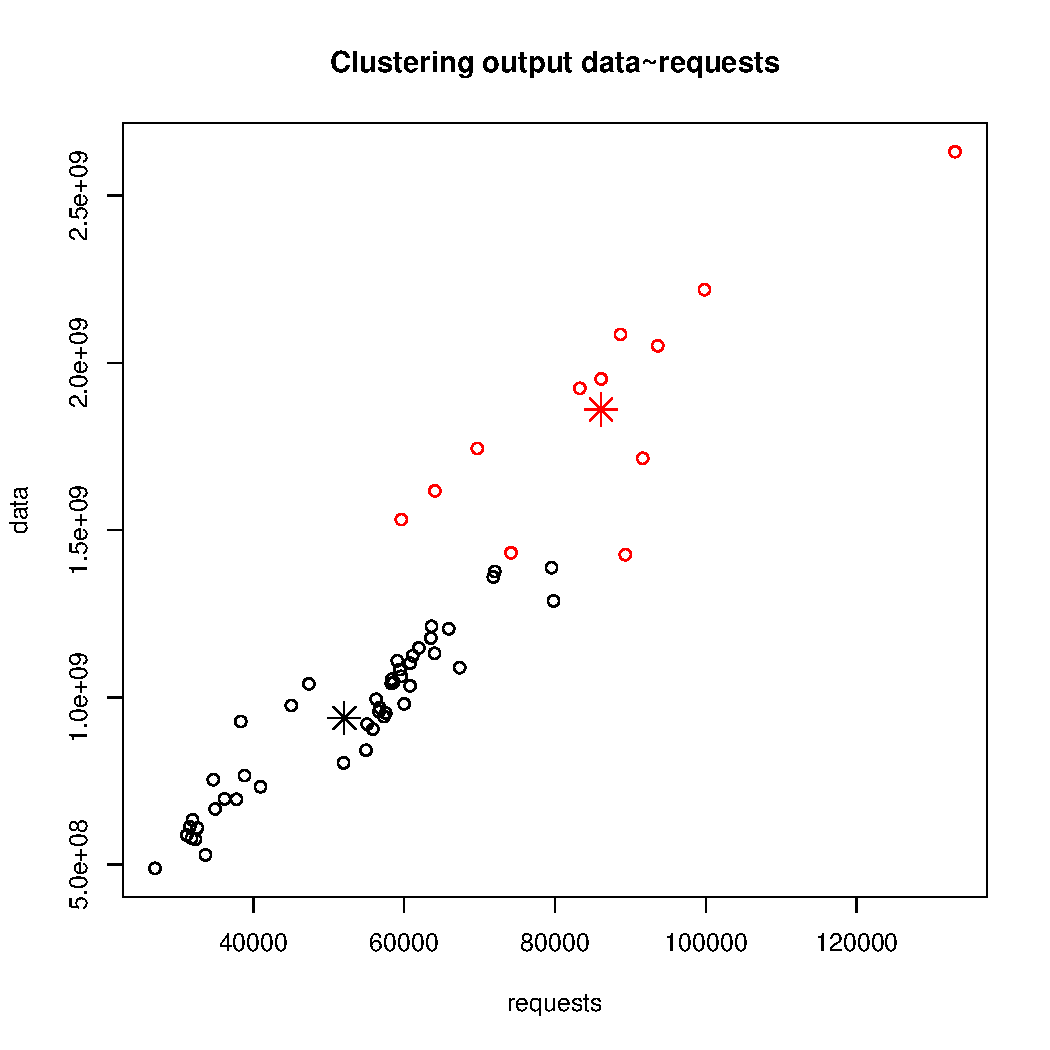
\includegraphics{Weblogs/ClusteringOutput1}}
\caption{Clustering output data requests relationships}
\end{figure}
\subsection{K-means}
I am going to use clustering algorithm called k-means nearest neighbours. The technique is centroid-based. The algorithm is very efficient if a number of clusters is known and clusters have convex shape, so our aim is perfectly fits for knn\footnote{k-means nearest neighbours}, picture 18 and 19.\\\\
In general the algorithm follows the steps:
\begin{enumerate}
\item centroid coordinates are randomly generated
\item elements of dataset are separated between centroids
\item centroid position is recalculated in according with average of the coordinates of assisted with the centroid elements 
\item repeat first three steps until centroid will not stop to change position
\end{enumerate}
\begin{figure}
\centerline{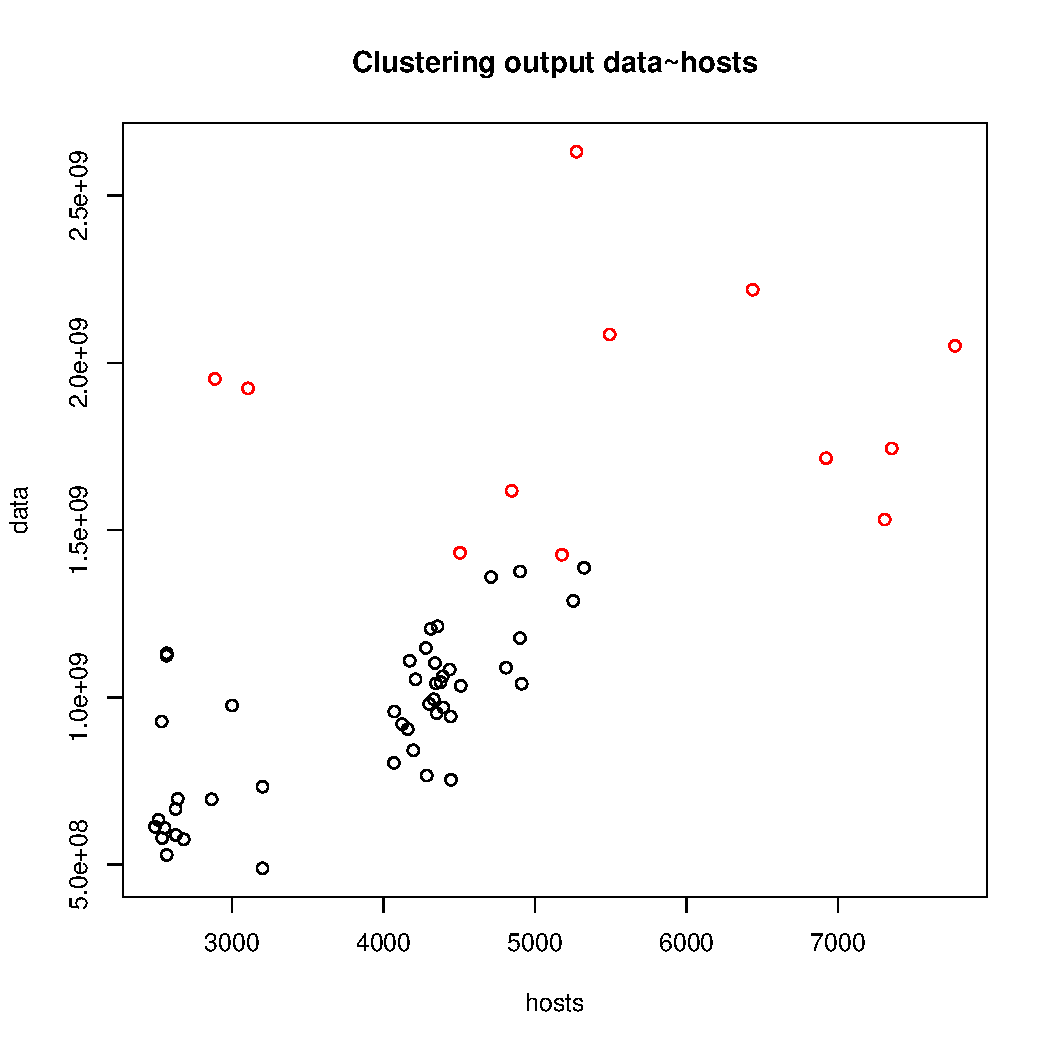
\includegraphics{Weblogs/ClusteringOutput2}}
\caption{Clustering output data hosts relationships}
\end{figure}
\subsection{Clustering of the weblogs}
I have made clustering into two clusters, with a knn algorithm, the output of the clustering is shown on the fig. 18 and 19. The centroids of the clusters are in a table 8. The clustering is very close to my expectations, so you can see that the amount of not "popular days" is bigger. The clustering is very stable - locations of centroids don't have noticeable changes if algorithm runs several times.
\begin{table}[H]
\caption{The centroids of the clusters}
\centerline{
\begin{tabular}{lccc}
\hline
 data & hosts & requests \\
\hline
959349519& 3887.583& 53292.29\\
1947266140 &5739.900 &86968.40\\
\end{tabular}}
\end{table}
\begin{lstlisting}
t<-cbind(data,hosts,requests)
k<-kmeans(t,2)
pdf("ClusteringOutput1.pdf")
plot(t[,3],t[,1],col=k$cluster,xlab="requests",
   ylab="data",main="Clustering output data~requests")
points(k$centers[,c(3,1)], col=1:2, pch=8, cex=2)
dev.off()
pdf("ClusteringOutput2.pdf")
plot(t[,2],t[,1],col=k$cluster,xlab="hosts",
    ylab="data",main="Clustering output data~hosts")
dev.off()
\end{lstlisting}
\section{Latex}
Latex is markup language especially popular scientific documents. The language allows to generate high quality pdf documents with complex formulas and graphs inside.  It has very simple syntax and plenty different packages for any possible situations and of course you can develop your own package.\\\\
I use Latex for the all my reports since Autumn and this report was not exception. The problem for me was to keep the beauty of R graphics inside Latex.
\subsection{Raster graphics}
Raster image contains an information about color of every dot separately, it is very good solution for complex images like photos, but it is not very good for graphs, because they lose quality after re-scaling. The best solution for raster graphics is PNG, because the compression algorithm is better for crispy edge than JPEG's one.
\subsection{Sweave}
Sweave is package which allows you to stream the power of R inside Latex. It is very basic in use tool, which helps you to write your R code inside *tex file and simply convert it into pdf with Latex compiler. It is the best solution for a small datasets, but unfortunately Sweave does not have an access to the full power of R, so it is not able to process really big datasets as we have, due to the problems with memory management.
\subsection{Vector graphics}
Vector image is built from different geometrical shapes with mathematical formulas. This technology is not able to show you realistic pictures, but it is extremely resizable and it makes the solution very good for graphs. R is able to save files into build into PDF vector images, which I can easily add to my Latex document. In my opinion it is the best way to combine R and Latex, but some times the PDF graphs can be very heavy, so probably it is better to convert graphs with huge number of data into raster graphics, if you want to have smooth scrolling of your documents, but I left everything in pdf.
\section{Conclusion}  
During the project I have improved my knowledge in R, stats, linear regression neural networks, clustering and Latex, it was also very helpful because it was my first experience with relatively big data, so I was able feel how  important is to write really efficient code. Despite the fact that some of my attempt was unsuccessful I get better understanding of the machine learning and how it can be applied for real life situations.
\newpage
\section{References:}
$[1]$ \href{http://gosset.wharton.upenn.edu/teaching/471/EPFL-Sweave-powerdot.pdf}{Sweave = R · LATEX\^2}(\today)\\\\
$[2]$ \href{http://scg.sdsu.edu/ann_r/}{Neural Networks (R)} (\today)\\\\
$[3]$ \href{https://www.otexts.org/fpp/9/3}{Neural network models} (\today)\\\\
$[4]$ \href{http://www.r-bloggers.com/using-neural-networks-for-credit-scoring-a-simple-example/}{Using neural networks for credit scoring: a simple example} (\today)\\\\
$[5]$ \href{http://www.statmethods.net/stats/regression.html}{Multiple (Linear) Regression} (\today)\\\\
$[6]$ \href{http://www.latex-project.org}{Latex - documentation} (\today)\\\\
$[7]$ Adaptive Neural Network Clustering of Web Users by Santosh K. Rangarajan, Vir V. Phoha, Kiran S. Balagani, Rastko R.Selmic Louisiana Tech University and S.S. Iyengar Louisiana State University(\today)\\\\
$[8]$ NASA-HTTP documentation about the weblogs(\today)\\\\
$[9]$ Neural Networks with R (\today)\\\\
$[10]$ k-means Clustering (\today)\\\\
$[11]$ \href{http://www.google.com/analytics/}{Google Analytics} (\today)\\\\
\newpage
\section{Appendix}
\begin{lstlisting}
readWeblogs<-function(file){
	weblogs<-read.table(file,fill=TRUE)
	colnames(weblogs)<-c("Host","Identification","Authuser","Time","TimeZone",
																			"Request","Status","Bytes")
	weblogs$Identification<-NULL
	weblogs$Authuser<-NULL
	weblogs$TimeZone<-NULL
	weblogs$Host[weblogs$Host=="-"] <- NA
	weblogs$Time[weblogs$Time=="-"] <- NA
	weblogs$Request[weblogs$Request=="-"] <- NA
	weblogs$Status[weblogs$Status=="-"] <- NA
	weblogs$Bytes[weblogs$Bytes=="-"] <- NA
	weblogs<-na.omit(weblogs)
	return(weblogs)
}

numberOf<-function(weblogs){
	numberOf=1
	data=as.character(sort(weblogs))
	for(i in 2:length(data))
	 if(data[i-1]!=data[i] || i==length(data))
	  numberOf=numberOf+1
	
	return(numberOf)
}

numberPer<-function(weblogs){
	numberOfBy=1
	data=as.character(sort(head(weblogs,n=length(weblogs)-1)))
	j=1
	for(i in 2:length(data)){
		if(data[i-1]!=data[i] || i==length(data)){
			j=j+1
			numberOfBy[j]=1
		}
		else numberOfBy[j]=numberOfBy[j]+1
	}
	return(numberOfBy)
}

weblogsMode <- function(x) {
  ux <- unique(x)
  ux[which.max(tabulate(match(x, ux)))]
}

mostFriqAmount<-function(weblogs){
	return(length(weblogs[ weblogsMode(as.character(weblogs))
				==as.character(weblogs)]))
}

hostsPerDay<-function(weblogs){
	day<-matrix(unlist(strsplit(as.character(na.omit(weblogs$Time)),split="/")),
						ncol=3, byrow=TRUE)[,1]
	start=1
	end=1
	result=0
	j=1
	for(i in 2:length(day))
		if(!is.na(day[i]) && !is.na(day[i-1])){
			if(day[i]!=day[i-1] || i==length(day)){
					 result[j]<-numberOf(weblogs$Host[start:end])
					 start<-end
					 j=j+1
					 }
			  else end=1+end
			  		}
	return(result)
}

requestsPerDay<-function(weblogs){
	day<-matrix(unlist(strsplit(as.character(na.omit(weblogs$Time)),split="/")),
					 ncol=3, byrow=TRUE)[,1]
	counter=0
	for(i in 2:length(day))
		if(!is.na(day[i]) && !is.na(day[i-1]) ){
			if(day[i]!=day[i-1])
					 counter[length(counter)+1]=1
			else counter[length(counter)]=1+counter[length(counter)]
			}
	return(counter)
}

dataPerHost<-function(weblogs){
	data<-as.numeric(as.character(weblogs$Bytes))
	data<-na.omit(data)

	numberOfHostsByNames=1
	hosts=as.character(sort(head(weblogs$Host,n=length(weblogs$Host)-1)))
	j=1
	for(i in 2:length(hosts))
		if(!is.na(data[i])){
			if(hosts[i-1]!=hosts[i] || length(hosts)==i){
				j=j+1
				numberOfHostsByNames[j]=0
			}
			else numberOfHostsByNames[j]=numberOfHostsByNames[j]+data[i]
	}
return(numberOfHostsByNames)
}

successfulRequests<-function(weblogs){
	status<-as.numeric(as.character(weblogs$Status))
	statusCounter=0
	for(i in 1:length(status))
		if(!is.na(status[i]))
			if(status[i]<400)
				 statusCounter=statusCounter+1
		 
	return(statusCounter)
}

unsuccessfulRequestsPerDay<-function(weblogs){
	day<-matrix(unlist(strsplit(as.character(na.omit(weblogs$Time)),split="/")), 
						ncol=3, byrow=TRUE)[,1]
	status<-as.numeric(as.character(weblogs$Status))
	statusCounter=0
	for(i in 2:length(status))
		if(!is.na(status[i]) && !is.na(day[i]) && !is.na(day[i-1]) ){
			if(day[i]!=day[i-1])
					 statusCounter[length(statusCounter)+1]=0
			  else if(status[i]>=400)
			  statusCounter[length(statusCounter)]=1+statusCounter[length(statusCounter)]
			}
	return(statusCounter)
}

dataAmount<-function(weblogs){
	data<-as.numeric(as.character(weblogs$Bytes))
	data<-na.omit(data)
	amount=0
		for(i in 1:length(data))
			if(!is.na(data[i]))
				if(data[i]>0)
					amount=amount+data[i]
	return(amount)
}

dataAmountPerDay<-function(weblogs){
	day<-matrix(unlist(strsplit(as.character(na.omit(weblogs$Time)),split="/")), 
							ncol=3, byrow=TRUE)[,1]
	data<-as.numeric(as.character(weblogs$Bytes))
	counter=0
	for(i in 2:length(data))
		if(!is.na(data[i]) && !is.na(day[i]) && !is.na(day[i-1]) ){
				if(day[i]!=day[i-1] || length(data)==i)
					 counter[length(counter)+1]=0
			 	else counter[length(counter)]=data[i]
			 	+counter[length(counter)]
			}
	return(counter)
}

mostPupolarRequestOfDay<-function(weblogs){
	day<-matrix(unlist(strsplit(as.character(na.omit(weblogs$Time)),split="/")),
														 ncol=3, byrow=TRUE)[,1]
	start=1
	end=1
	mostPopRequest=''
	j=1
	for(i in 2:length(day))
		if(!is.na(day[i]) && !is.na(day[i-1])){
			if(day[i]!=day[i-1] || i==length(day)){
					 mostPopRequest[j]
			<-as.character(weblogsMode(weblogs$Request[start:end]))
					 start<-end
					 j=j+1
					 }
			  else end=1+end
			  		}
	return(mostPopRequest)
}

mostPupolarRequestOfDayAmount<-function(weblogs){
	day<-matrix(unlist(strsplit(as.character(na.omit(weblogs$Time)),split="/")), 
					ncol=3, byrow=TRUE)[,1]
	start=1
	end=1
	mostPopRequest=0
	j=1
	for(i in 2:length(day))
		if(!is.na(day[i]) && !is.na(day[i-1])){
			if(day[i]!=day[i-1] || i==length(day) || length(day)==i){
					 data<-as.character(weblogs$Request[start:end])
					 mostPopRequest[j]
					 <-length(data[weblogsMode(data)==data])
					 start<-end
					 j=j+1
					 }
			  else end=1+end
			  		}
	return(mostPopRequest)
}

mostPupolarRequestOfDayName<-function(weblogs){
	day<-matrix(unlist(strsplit(as.character(na.omit(weblogs$Time)),split="/")), 
							ncol=3, byrow=TRUE)[,1]
	start=1
	end=1
	mostPopRequest=0
	j=1
	for(i in 2:length(day))
		if(!is.na(day[i]) && !is.na(day[i-1])){
			if(day[i]!=day[i-1] || i==length(day) || length(day)==i){
					 data<-as.character(weblogs$Request[start:end])
					 mostPopRequest[j]<-data[weblogsMode(data)==data]
					 start<-end
					 j=j+1
					 }
			  else end=1+end
			  		}
	return(mostPopRequest)
}

mostActiveHostOfDayAmount<-function(weblogs){
	day<-matrix(unlist(strsplit(as.character(na.omit(weblogs$Time)),split="/")),
					ncol=3, byrow=TRUE)[,1]
	start=1
	end=1
	mostPopHost=0
	j=1
	for(i in 2:length(day))
		if(!is.na(day[i]) && !is.na(day[i-1])){
			if(day[i]!=day[i-1] || i==length(day) || length(day)==i){
					 data<-as.character(weblogs$Host[start:end])
					 mostPopHost[j]
					 <-length(data[weblogsMode(data)==data])
					 start<-end
					 j=j+1
					 }
			  else end=1+end
			  		}
	return(mostPopHost)
}

mostActiveHostOfDayName<-function(weblogs){
day<-matrix(unlist(strsplit(as.character(na.omit(weblogs$Time)),split="/")),
						ncol=3, byrow=TRUE)[,1]
start=1
end=1
mostPopHost=''
j=1
for(i in 2:length(day))
	if(!is.na(day[i]) && !is.na(day[i-1])){
		if(day[i]!=day[i-1] || i==length(day) || length(day)==i){
				 data<-as.character(weblogs$Host[start:end])
				 mostPopHost[j]
				 <-as.character(data[weblogsMode(data)==data])
				 start<-end
				 j=j+1
				 }
		  else end=1+end
		  		}
return(mostPopHost)
}

analitics1<-function(r){
	print("Number of hosts")
	print(numberOf(r$Host))
	print("Number of requests")
	print(length(r$host))
	print("Most popular request names")
	print(weblogsMode(r$Request))
	print("Most popular request amount")
	print(mostFriqAmount(r$Request))
	print("Most active host names")
	print(weblogsMode(r$Host))
	print("Most active host amount")
	print(mostFriqAmount(r$Host))
	print("Most active host per day names")
	print(mostActiveHostOfDayName(r))
	print("Number of resourses")
	print(numberOf(r$Request))
	print("Amount of transferred data")
	print(dataAmount(r))
	print("The biggest package")
	print(max(as.numeric(as.character(r$Bytes)), na.rm = TRUE))
	print("Most popular request of day names")
	print(mostPupolarRequestOfDay(r))
	
	
	plot(numberPer(r$Host),main="Number of requests per host",
			xlab="Host",ylab="Request")
	dev.new()
	plot(hostsPerDay(r),main="Number of hosts per day",
				xlab="Day",ylab="Host")
	dev.new()
	plot(mostActiveHostOfDayAmount(r),main="Most active host per day amounts",
						xlab="Day",ylab="Request")
	dev.new()
	plot(requestsPerDay(r),main="Number of requests per day",
						xlab="Day",ylab="Request")
	dev.new()
	plot(numberPer(r$Request),main="Number of number requests per recourse",
			xlab="Recourse",ylab="Request")
	dev.new()
	plot(mostPupolarRequestOfDayAmount(r),main="Most popular request of day  amounts",
				xlab="Day",yla="Request")
	dev.new()
	plot(dataAmountPerDay(r),main="Data per day",xlab="Day",ylab="Data")
	dev.new()
	plot(dataPerHost(r),main="Data per host",xlab="Host",ylab="Data")
}
analitics2<-function(r){
	print("Number of hosts")
	print(numberOf(r$Host))
	print("Most popular request names")
	print(weblogsMode(r$Request))
	print("Most popular request amount")
	print(mostFriqAmount(r$Request))
	print("Most active host names")
	print(weblogsMode(r$Host))
	print("Most active host amount")
	print(mostFriqAmount(r$Host))
	print("Most active host per day names")
	print(mostActiveHostOfDayName(r))
	print("Number of requests")
	print(numberOf(r$Request))
	print("Amount of transferred data")
	print(dataAmount(r))
	print("The biggest package")
	print(max(as.numeric(as.character(r$Bytes)), na.rm = TRUE))
	print("Most popular request of day names")
	print(mostPupolarRequestOfDay(r))
	
	pdf("NumberOfRequestsPerhost.pdf")
	plot(numberPer(r$Host),main="Number of requests per host",
			xlab="Host",ylab="Request")
	dev.off()
	pdf("NumberOfHostsPerDay.pdf")
	plot(hostsPerDay(r),main="Number of hosts per day",
			xlab="Day",ylab="Host")
	dev.off()
	pdf("MostActiveHostPerDayAmounts.pdf")
	plot(mostActiveHostOfDayAmount(r),main="Most active host per day amounts",
					xlab="Day",ylab="Request")
	dev.off()
	pdf("NumberOfRequestsPerDay.pdf")
	plot(requestsPerDay(r),main="Number of requests per day"
				,xlab="Day",ylab="Request")
	dev.off()
	pdf("NumberOfNumberRequestsPerRecourse.pdf")
	plot(numberPer(r$Request),main="Number of number requests per recourse",	
			xlab="Recourse",ylab="Request")
	dev.off()
	pdf("MostPopularRequestOfDayAmounts.pdf")
	plot(mostPupolarRequestOfDayAmount(r),main="Most popular request of day amounts",
				xlab="Day",yla="Request")
	dev.off()
	pdf("DataPerDay.pdf")
	plot(dataAmountPerDay(r),main="Data per day",xlab="Day",ylab="Data")
	dev.off()
	pdf("DataPerHost.pdf")
	plot(dataPerHost(r),main="Data per host",xlab="Host",ylab="Data")
	dev.off()
}

\end{lstlisting}
\end{document}
